\documentclass[12pt,fleqn]{report} %taille de la police par défaut, et équations jusitifées à gauche
\usepackage{blindtext} % Package to generate dummy text throughout this template 

\usepackage{mathptmx}
%\usepackage[sc]{mathpazo} % Use the Palatino font
\usepackage[T1]{fontenc} % Use 8-bit encoding that has 256 glyphs
\linespread{1.05} % Line spacing - Palatino needs more space between lines
\usepackage{microtype} % Slightly tweak font spacing for aesthetics

\usepackage[english]{babel} % Language hyphenation and typographical rules

\usepackage[hmarginratio=1:1,left=15mm,right=15mm,top=32mm,columnsep=20pt]{geometry} % Document margins
\usepackage[hang, small,labelfont=bf,up,textfont=it,up]{caption} % Custom captions under/above floats in tables or figures
\usepackage{booktabs} % Horizontal rules in tables

\usepackage{lettrine} % The lettrine is the first enlarged letter at the beginning of the text

\usepackage{enumitem} % Customized lists
\setlist[itemize]{noitemsep} % Make itemize lists more compact

\usepackage{abstract} % Allows abstract customization
\renewcommand{\abstractnamefont}{\normalfont\bfseries} % Set the "Abstract" text to bold
\renewcommand{\abstracttextfont}{\normalfont\small\itshape} % Set the abstract itself to small italic text

\usepackage{titlesec} % Allows customization of titles
\renewcommand\thesection{\Roman{section}} % Roman numerals for the sections
\renewcommand\thesubsection{\roman{subsection}} % roman numerals for subsections
\titleformat{\section}[block]{\large\scshape\centering}{\thesection.}{1em}{} % Change the look of the section titles
\titleformat{\subsection}[block]{\large}{\thesubsection.}{1em}{} % Change the look of the section titles

\usepackage{fancyhdr} % Headers and footers
\pagestyle{fancy} % All pages have headers and footers
\fancyhead{} % Blank out the default header
\fancyfoot{} % Blank out the default footer
\fancyfoot[RO,LE]{\thepage} % Custom footer text

\usepackage{titling} % Customizing the title section

\usepackage{booktabs}       % pour de jolis tableaux
%\usepackage{fancyhdr}       % pour des entêtes et pieds de pages améliorés.
\usepackage{makeidx}        % requis pour faire les index
\usepackage{amsmath}
\usepackage{amssymb}
\usepackage{mathtools}
\usepackage{amsfonts}
\usepackage{amssymb}
\usepackage{color}
\usepackage{array}
\usepackage{graphicx}
\usepackage{animate}
\usepackage{caption} 
\usepackage{hyperref}
\usepackage{algorithm}
\usepackage{algorithmic}
\usepackage{subcaption}
\usepackage{times}
\usepackage{tabularx}
\usepackage{authblk}
\usepackage{multirow}
\usepackage{array}

\providecommand{\keywords}[1]{\textbf{\textit{keywords :}} #1}
\renewcommand{\thesubsection}{\Alph{subsection}}

     % Ce fichier contient tous les packages nécessaires à la compilation
\makeindex           % donne l'ordre de créer l'index

\begin{document}


\renewcommand{\contentsname}{Sommaire}%
\renewcommand{\listfigurename}{Table des figures}%
\renewcommand{\listtablename}{Table des tableaux}%
\renewcommand{\bibname}{Bibliographie}  % des jolis noms pour les sections bibliographiques


%----------------------------------------------------------------------------------------
%	 PAGE DE TITRE
%----------------------------------------------------------------------------------------

\begingroup
\thispagestyle{empty}
\AddToShipoutPicture*{\put(6,5){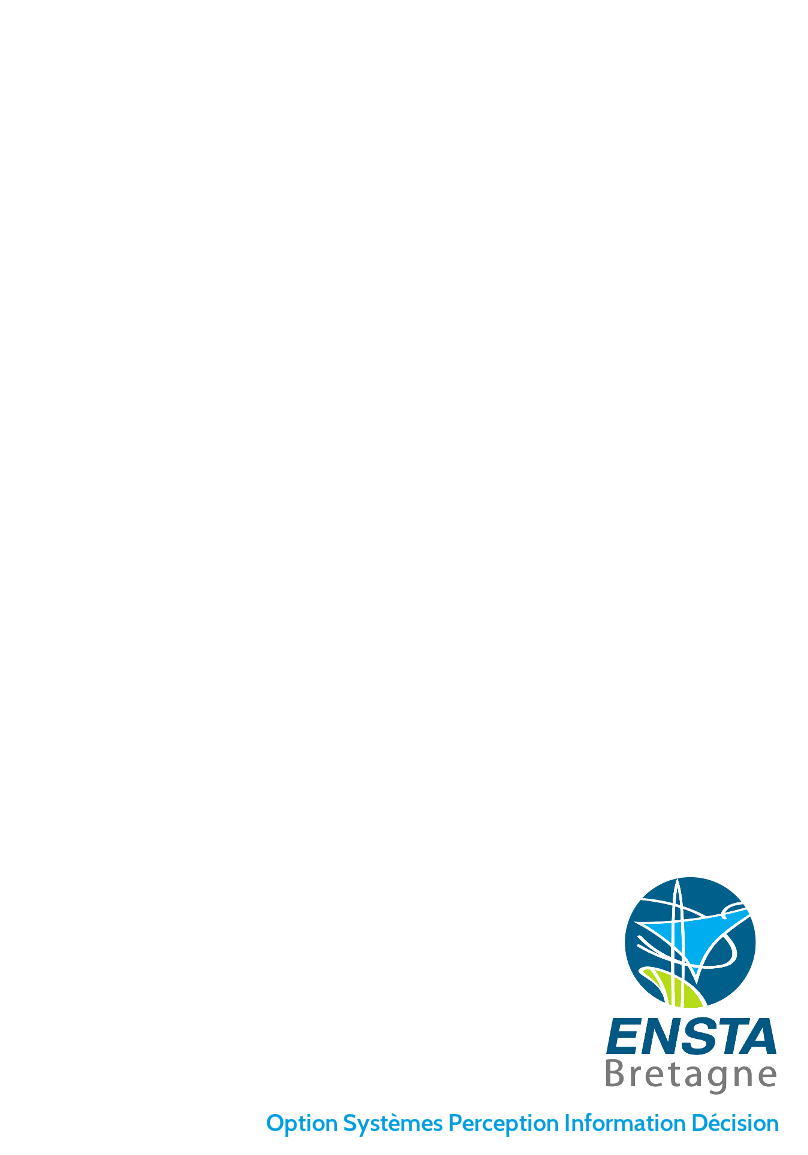
\includegraphics[scale=1]{Images/FondTitreSPID}}} % Image background
\begin{center}
\vspace*{2cm}
{\Huge \textsc{\textbf{Rapport projet de fin d'étude}}}\\


\vspace*{2cm}
{\huge Réalisation d'un programme d'aide au diagnostic, application sur les pathologies cérébrales.}\par % Intitulé du projet
\end{center}
%\begin{figure}[H]
%\centering
%    \includegraphics[trim={1cm 1cm 0.7cm 5cm},clip, scale=0.6]{biscay.png}
%\end{figure}

\vspace*{1.5cm}
\textbf{\large Écrit par:} 
\begin{center}
{\huge 
\begin{tabular}{cc}
\\
Philippe Chuzel\\
\\
Promotion 2016, option SPID Robotique
\end{tabular}}
\end{center}


\vspace*{0.5 cm}
{\large \textbf{Sous la supervision de :}}\\
\begin{center}
{\large
Ali Mansour}
\end{center}

\vspace*{0.5 cm}
\begin{center}
{\large
ENSTA Bretagne}
\end{center}
\endgroup


\afterpage{\null\newpage}

%----------------------------------------------------------------------------------------
%	Remerciment
%----------------------------------------------------------------------------------------

\chapter*{Remerciement}
Je tiens à remercier ici M. Ali Mansour et M. Cexus pour m'avoir aidé à trouver ce PFE en rapport avec les problématiques de la santé. Ce stage fut riche en rencontre très intéressante et ce fut un plaisir de travailler avec les contacts que j'ai pu avoir dont notamment les chercheurs de l'INSERM et les médecins du CHRU de Brest.

Je remercie donc M. Nacim Betrouni et M. Denis Hamad pour leurs conseils et leur accueil au sein de l'INSERM de Lille. Je remercie également les Médecins M. Jean Christophe Gentrix et M. Julien Ognard pour leurs aide et conseils sur l'analyse des images médicales. Je leur dois aussi toute la base de données d'image à laquelle j'ai pu avoir accès.

Ce fut un projet avec peu de rapport avec les thématiques que j'ai pu étudier à l'ENSTA mais je me rends compte à quel point les compétences et expériences que j'ai eu tant pendant mon année militaire que pendant ma formation de trois ans à l'ENSTA m'ont permis d'aboutir à ce résultat. Je tiens donc à remercier tout les professeurs de l'ENSTA pour les cours qu'ils nous ont fait.

J'ai remercie encore une fois M. Ali Mansour pour m'avoir permis de publier, sa patience pour les relectures, le stylo rouge qu'il a sacrifié pour cette tache et la liberté de mouvement qu'il m'a laissé pendant ce PFE afin que je puisse également me former sur d'autres thématiques.

%----------------------------------------------------------------------------------------
%	SOMMAIRE
%----------------------------------------------------------------------------------------
\tableofcontents  % Imprime le sommaire
%\listoftables   % table des tableaux
\cleardoublepage  % pour commencer sur une page impaire

%\chapter*{Abstract}
%\input{Abstract}

\chapter*{Introduction}
Physicians use different sources of images in order to make a diagnostic. In the last two decades, many studies have been made in order to automatise the identification and the characterisation of disease by extracting relevant information from those sources of images like the MRI, the Elastography or the Echography, in order to propose help to diagnostic \cite{tartare2014contribution}, \cite{schmitt2011characterization}, \cite{schmitt2013shear}, \cite{ophir1991elastography}.

In \cite{tartare2014contribution}, a new methodology was proposed in order to realise an automatic segmentation of tumour tissues for prostate cancer. Our objective is to generalise and modify the previously proposed method to improve the segmentation of MRI images to diagnose brain pathologies.

Our project focuses on the perfusion MRI by using a spectral clustering algorithm. Physicians use perfusion MRI in order to check the variation of pixel intensity of the MRI image and identify abnormal behaviour. To apply similar methodology, we have to develop a unsupervised classification approach. The main issue is that many classification algorithms like the k-means are not suitable for signal classification. The main purpose of spectral clustering is to firstly estimate the similarity among signals and, build a similarity matrix and work on the eigenvector and eigenvalue of this matrix in order to perform a classification. Spectral clustering algorithms are the most adapted for the data we are dealing with.

This study is the result of a collaboration among four institutes: ENSTA Bretagne, Brest Hospital university Research Center (CHRU), INSERM of Lille and ULCO.

We apply our approach on a perfusion MRI database of twelve patients showing different pathologies in the brain in order to apply our algorithm.Those MRI have been provided by the Brest CHRU. An example of MRI images obtained can be seen in the figure \ref{fig:diffusion}. For each pixel, a variation of the intensity on the different MRI images can be observe.

\begin{figure}
\centering
\begin{subfigure}[t]{0.22\textwidth}
\centering
    \vspace{0.00\textheight}
    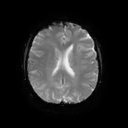
\includegraphics[scale=0.9,angle=0]{Im1.png}
    \caption{MRI without contrast product}
    \label{fig:without} 
\end{subfigure}
\begin{subfigure}[t]{0.22\textwidth}
\centering
    \vspace{0.00\textheight}
    \includegraphics[scale=0.9,angle=0]{Im7.png}
    \caption{beginning of the diffusion}
    \label{fig:First} 
\end{subfigure}
\begin{subfigure}[t]{0.22\textwidth}
\centering
    \vspace{0.00\textheight}
    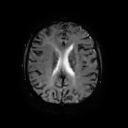
\includegraphics[scale=0.9,angle=0]{Im8.png}
    \caption{Peak of diffusion}
    \label{fig:Second} 
\end{subfigure}
\begin{subfigure}[t]{0.22\textwidth}
\centering
    \vspace{0.00\textheight}
    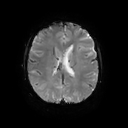
\includegraphics[scale=0.9,angle=0]{Im13.png}
    \caption{end of the diffusion}
    \label{fig:Last} 
\end{subfigure}
    \caption{Diffusion of the contrast product on the MRI.}
    \label{fig:diffusion} 
\end{figure}

%At the beginning, we wanted to apply those results for detection and the characterisation of the thrombus and the deep venous thrombosis. Many options are studied in order to achieve this goal like the use of Elastography and echography \cite{schmitt2011characterization}, \cite{schmitt2013shear}, \cite{ophir1991elastography}.We wanted to apply this methodology which use the MRI images as a new source of information on the clot. Nevertheless, we arrived quickly to those results:
%
%\begin{itemize}
%
%\item The MRI signature of the clot is highly dependent on its age, its composition and surrounding tissues.
%
%\item The position of the clot is not fixed. The clot can be naturally dissolved. 
%
%\item The composition of the clot can be known only through an extraction from the patient, which is not always possible. 
%
%\end{itemize}





%----------------------------------------------------------------------------------------
%	PART I 
%----------------------------------------------------------------------------------------
\part{Présentation de la problématique du projet de fin d'étude.}
\chapter{Quelles sont les sources d'informations exploitables?}


Le sujet de départ de l'étude, qui est mené actuellement à l'ENSTA Bretagne, est de proposer des méthodes d'identification et de caractérisation de la thrombose et du thrombose veineuse profonde ou DVT. Cette étude est menée en partenariat avec plusieurs medecins du CHRU de Brest, M. Bressollette et M. Moittier qui fournissent actuellement la majorité des images qui sont utilisées pour cette étude. Dans un premier temps, nous nous sommes intéressés aux différents types d'image que nous pouvions avoir accès. 


\section{Elastométrie}

L'élastométrie est une méthode d'acquisition d'image médicale non invasive et très pratique. En effet, très facile à mettre en œuvre et peu couteuse en temps et en argent. Cette méthode consiste à créer une représentation d'une zone du corps à partir de l'élasticité du tissu biologique \cite{ophir1991elastography}.

\begin{figure}[H]
\centering
    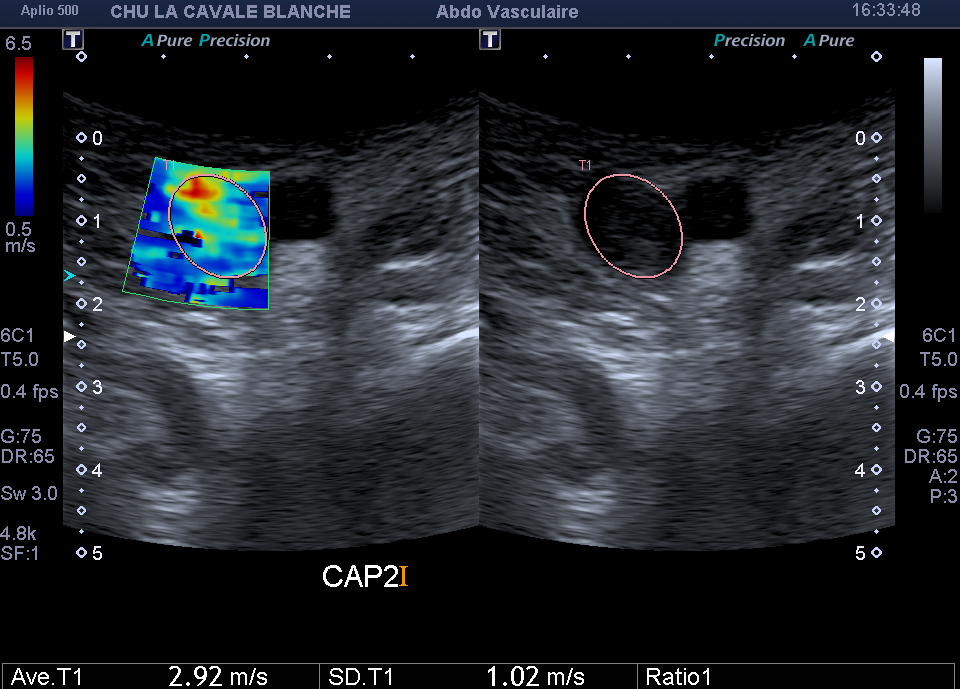
\includegraphics[scale=0.3,angle=0]{Images/ExempleElastometrie.png}
    \caption{Exemple d'image d'élastometrie.}
    \label{fig:ExempleElastometrie}
\end{figure}

Cette méthode présente plusieurs particularités pour cette étude:

\begin{itemize}
\item Elle est très facile à utiliser et se fait en un temps très faible. 
\item C'est une méthode qui n'est pas invasive.
\item Bien que la mise en œuvre soit facile, les images obtenues sont de médiocre qualité en terme de résolution.
\end{itemize}

Néanmoins, il y a un problème à cette méthode. Il est nécessaire de définir un protocole unique à tous les patients pour faire en sorte que les images obtenues par ce procédé soient comparables.

 
\section{Échographie}

L'échographie est une technique d'imagerie qui consiste à utiliser des ondes ultrasons. En fonction des propriétés du milieu, certains tissus ou partie du corps apparaitront en noir, gris ou blanc. 

\begin{figure}[H]
\centering
    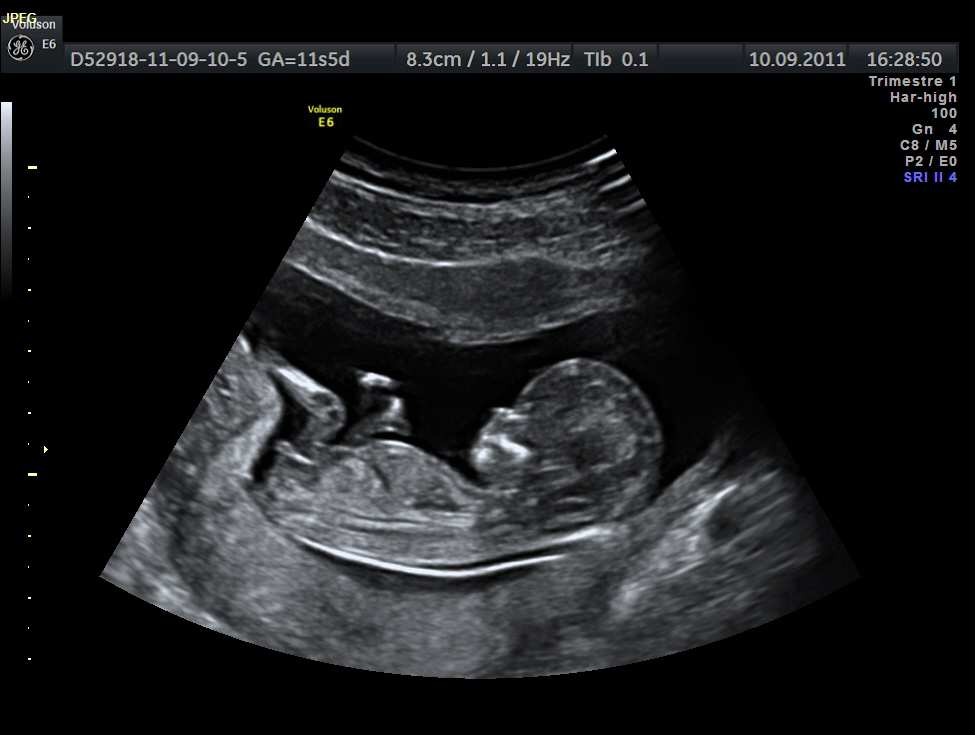
\includegraphics[scale=0.6,angle=0]{Images/Echographie-profil.jpg}
    \caption{Exemple d'image échographique pour l'obstétrie.}
    \label{fig:Echographie}
\end{figure}

Cette méthode présente les mêmes avantages que l'élastométrie. Elle est peu chère, facile à mettre en œuvre et non invasive pour le patient. Néanmoins, elle présente également des images de très faible qualité en terme de résolution.


\section{Computed tomography angiography / Angiographie}

L'angiographie est une technique d'imagerie qui est invasive. Bien qu'elle présente plusieurs intérêts, notamment car elle consiste à faire une imagerie des vaisseaux sanguins par rayon X (veines ou artères), il y a plusieurs effets secondaires (vomissement, vertiges, nausées, réactions allergiques, saignement important...) ou contre-indications (grossesse, tension artérielle trop basse...). Cette piste ne sera pas étudiée ici.

\begin{figure}[H]
\centering
    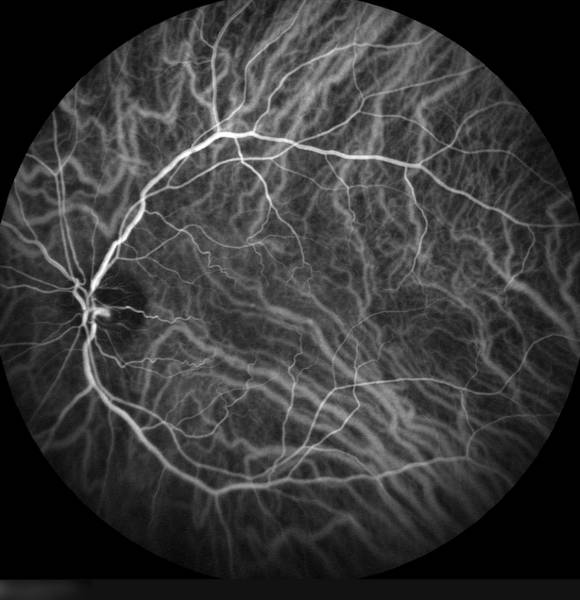
\includegraphics[scale=0.4,angle=0]{Images/m_1407858437.jpg}
    \caption{Exemple d'angiographie pour l'œil.}
    \label{fig:m_1407858437}
\end{figure}

\section{Scanner}

Le scanner est un outil qui propose de reconstituer des images des tissus par ordinateur à partir des différences d'absorption des rayons X. Ce procédé permet d'obtenir des coupes du corps du patient très rapidement et présente certains avantages et inconvénients. C'est une méthode qui permet d'obtenir très rapidement des images médicales exploitable pour faire un diagnostic. Néanmoins, c'est un procédé qui impose l'utilisation de rayon X donc irradiant. C'est donc un procédé invasif.


\begin{figure}[H]
\centering
    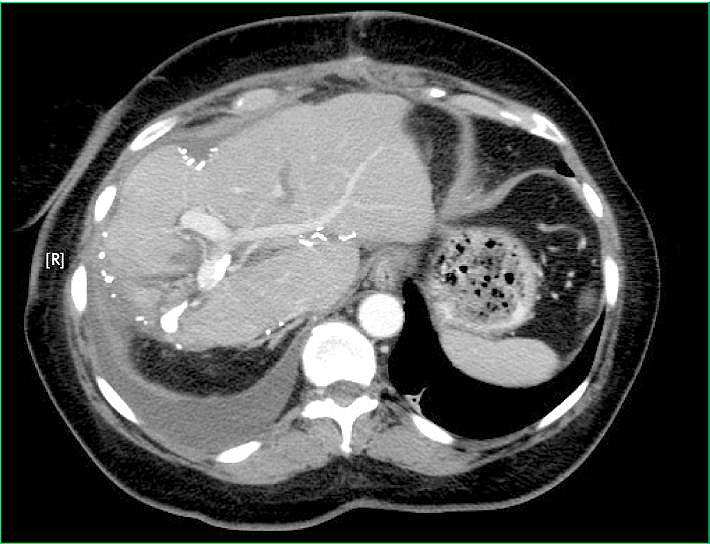
\includegraphics[scale=0.4,angle=0]{Images/Scanner.jpg}
    \caption{Exemple d'image issue d'un scanner.}
    \label{fig:m_1407858437}
\end{figure}

\section{IRM}

L'IRM ou l'imagerie par résonance magnétique sera ici la source d'image médicale qui sera étudiée. Elle produit des images avec une haute résolution et présent un énorme avantage pour nous. C'est un procédé entièrement non invasif et, à la différence du scanner, elle ne nécessite aucun produit irradiant.

\begin{figure}[H]
\centering
    \includegraphics[scale=2,angle=0]{Images/Im7.png}
    \caption{Exemple d'image IRM.}
    \label{fig:m_1407858437}
\end{figure}

Le principe de base de l'IRM est de faire une imagerie des atomes d'hydrogène présent dans le tissu que nous souhaitons étudier. Nous considérons ici que le noyau de l'atome d'hydrogène qui est juste un proton qui tourne sur lui-même. L'idée est d'utiliser un puissant aimant qui va générer un champs et une onde radio excitatrice de fréquence identique à la fréquence de rotation des protons. Ceci a pour conséquence que tous les protons tournent dans un même axe qui est légèrement différent de l'axe du champs de l'aimant et qu'ils soient en phase. Ce léger écart dans l'orientation de l'axe est dû à l'excitation par l'onde radio.

A partir de ce point, on coupe l'onde excitatrice et deux phénomènes se présentent:

\begin{itemize}
\item Les protons vont revenir à leur état chaotique de départ et vont tous se déphaser,
\item Les protons vont tous s'orienter par rapport à l'axe du champs de l'aimant.
\end{itemize}

Ce changement d'état se traduit par la diffusion d'un signal qui est capté et permet la réalisation de la cartographie des protons et donc de notre image IRM. On peut paramétrer la machine pour mesurer deux paramètres:

\begin{itemize}
\item Soit on mesure le temps que mettent les protons pour se remettre dans l'axe de l'aimant ce qui est appelé temps de relaxation T1 ou pondération T1.
\item Soit on mesure le temps que mettent les protons pour se désynchroniser ce qui est appelé temps de relaxation T2 ou pondération T2.
\end{itemize}


\chapter{Premier sujet: Caractérisation de la thrombose par les IRM}


Pendant la durée du stage, nous étions deux à travailler sur la problématique de la détection et de la caractérisation de la thrombose. Thibaud Berthomier qui est actuellement en thèse à l'ENSTA Bretagne a pu récupérer de la part du CHRU plusieurs images de caillot sanguin. L'étude qu'il mène se concentre sur les caillots situés au niveau de la cuisse. Je devais, pour ma part, explorer une autre piste qui consistait à utiliser des images IRM. Je devais également utiliser le résultat d'une thèse pour voir si la méthode qui y est dévellopée pouvait être utilisée \cite{tartare2014contribution}, \cite{tartare2014spectral}. Il nous a fallu donc dans un premier temps faire un état de l'art sur les éléments développés dans cette thèse et sur le thrombose veineuse profonde (DVT).


\section{Première piste, utilisation des IRM de perfusion.}

Le principe de l'IRM de perfusion est d'injecter un produit de contraste, ici le galonium, qui est visible par IRM et de voir comment ce produit se diffuse au cours du temps dans les différentes zones du corps. A terme, nous obtenons un ensemble d'image traduisant l'évolution de la concentration du produit dans la zone étudiée au cours du temps. A partir de ces images, nous pouvons déterminer la courbe d'intensité au cours du temps de chaque pixel de l'IRM. L'idée est donc de voir le comportement d'une zone du corps avant, pendant et après injection du produit de contraste et de voir si on peut caractériser ainsi une zone en particulier.

Dans un premier temps, nous souhaitions utiliser la méthodologie mise au point dans la thèse \cite{tartare2014contribution}. Cette dernière propose deux outils pour l'aide au diagnostic. Le premier est l'établissement de carte de paramètre pharmacocinétique. Le second est l'utilisation d'algorithme de classification non supervisé pour réaliser des clusters à partir différentes courbes d'intensité obtenues afin d'isoler les courbes présentant le même comportement entre elles. Ainsi, on obtient une nouvelle carte segmentée qui indique les régions qui présentent les même caractéristiques.

\begin{figure}[H]
\centering
    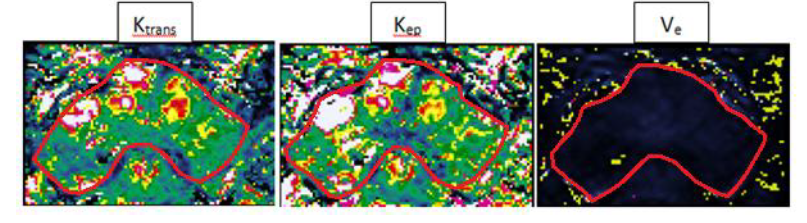
\includegraphics[scale=0.6,angle=0]{Images/CatreDeParametresPharmacocinetique.png}
    \caption{Cartes de parametre pharmacocinetique $K_p, K_{trans}$ et $V_e$ de la prostate.}
    \label{fig:CarteDeParametresPharmacocinetique}
\end{figure}

La figure qui suit montre la méthodologie appliquée ici \ref{fig:Classif}.
 
\begin{figure}[H]
\centering
    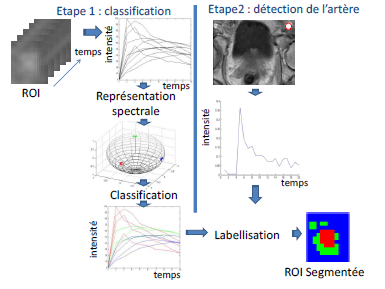
\includegraphics[scale=1,angle=0]{Images/Classif.png}
    \caption{Méthodologie suivie pour la classification.}
    \label{fig:Classif}
\end{figure}

L'idée est d'avoir au final des images qui segmentent directement les tissus sains et les tissus pathologiques.

\section{Qu'est ce que la thrombose veineuse profonde}

On appelle thrombose le fait qu'un caillot sanguin ou thrombus se développe à l'intérieur d'un vaisseau sanguin. Il peut être soit artériel, soit veineux. Dans les deux cas, ce caillot peut obstruer le vaisseau et donc empêcher la circulation du sang.

\begin{figure}[H]
\centering
    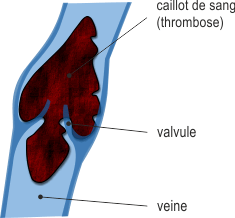
\includegraphics[scale=2,angle=0]{Images/phleb1.png}
    \caption{Exemple illustrant la thrombose.}
    \label{fig:phleb1}
\end{figure}

La phlébite est un cas de thrombose veineuse pour une veine profonde et est consécutif à l'inflammation de la veine et au risque de déplacement du caillot. D'où le terme de thrombose veineuse profonde DVT (deep venous thrombose).

Parmi les principales causes, nous pouvons énumérer:


\begin{itemize}
\item Une lésion dans une veine qui entraine une coagulation au niveau du tissu sanguin (blessure...),
\item Certains paramètres génétiques qui peuvent favoriser le processus de thrombose,
\item Les périodes prolongées dans une même position (alitement, accouchement, voyage long en avion...),
\item Des précédentes expériences traumatisantes pour le corps (cancer, opération...),
\item Influence de certaines substances sur la paroi des artères (tabac, médicaments...), 
\item Facteurs favorisant la formation de thrombus (obésité, diabète, hypercholestérolémie...). 
\end{itemize}

Une fois le caillot formé, il peut se produire différents phénomènes:

\begin{itemize}
\item Il peut de lui même se désagréger et disparaitre naturellement,
\item Il peut se calcifier ou changer de structure se qui peut amener à la formation de pelote fibreuse,
\item Il peut se détacher et atteindre un des vaisseaux pulmonaires. Ceci se traduit par une embolie pulmonaire qui s'avère très dangereux.
\end{itemize}

Dans tous les cas, la présence de ce caillot dans le système circulatoire sanguin d'un patient peut mener à des perturbations graves du flux sanguin avec l'apparition d'œdème ou d'ulcère pour la zone inférieure du corps que nous allons étudier.

\section{Problème rencontré vis à vis des IRM de thrombus.}

Les premières semaines du stage ont donc consisté à tenter de récupérer des images IRM de thrombus afin de voir ce qui était possible de faire. Très rapidement, plusieurs problèmes se sont présentés:

\begin{itemize}
\item Le fait d'utiliser des IRM pour des caillots sanguins est encore très récent et nécessite la création de nouveaux protocoles qui doivent être validés par des comités d'éthique. Cette démarche prend beaucoup de temps et cette utilisation des IRM reste encore au niveau de la recherche expérimentale.
\item Il n'y a pour l'instant aucune image IRM de caillot situé au niveau de la cuisse, caillot qui est pour l'instant principalement étudié.
\item Pour les thrombus cérébraux, il existe des IRM mais plusieurs problèmes se sont rapidement manifestés. La signature IRM du caillot change assez rapidement en fonction de son âge. De plus, sa composition et sa position ont un lourd impact sur comment il sera vu sur l'IRM.
\end{itemize}

Au final, si nous devions poursuivre sur cette voie, nous aurions dû nous concentrer sur les thromboses cérébraux. De plus, après plusieurs discussions avec les médecins du CHRU, cela aurait nécessité un travail qui n'était pas réalisable en 6 mois.

\chapter{Changement de sujet: Réalisation d'un programme d'aide au diagnostic pour les pathologies cérébrales.}


Après une période d'investigation qui a démontré que le premier objectif était irréalisable dans le temps imparti, les médecins du CHRU m'ont proposé de réaliser un programme d'aide au diagnostic pour les pathologies cérébrales. Ces derniers étaient justement spécialisés sur cette partie du corps humain et pouvaient me fournir les images nécessaires pour que je puisse travailler. 
De plus, j'ai pu prendre contact avec les personnes qui ont encadré la thèse sur laquelle je m'appuyais pour récupérer leurs données expérimentales et simulées. J'ai donc pu déjà profiter de leur expertise et d'autre part récupérer plusieurs données simulées de prostate présentant des tumeurs et plusieurs IRM de perfusion de prostate présentant cette pathologie.

\begin{figure}[H]
\centering
    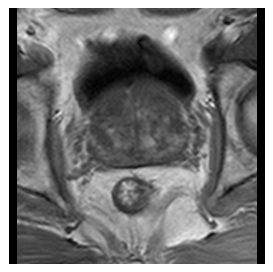
\includegraphics[scale=1,angle=0]{Images/ProstateImage.png}
    \caption{Image IRM de la prostate.}
    \label{fig:ProstateImage}
\end{figure}

Au final, j'ai pu récupérer avec le CHRU les IRM de perfusion de 13 patients présentant des pathologies assez visibles pour que je puisse tester mes algorithmes. Parmi les pathologies qui ont été recensées, il y a plusieurs formes de cancer et des œdèmes assez significatifs. Le travail qui va suivre a donc pour but de voir quelles sont les pathologies qui peuvent être identifiées par cette méthode, généraliser et proposer des améliorations au niveau de la chaine de traitement et donc réaliser un programme d'aide au diagnostic pour ces pathologies.






%----------------------------------------------------------------------------------------
%	PART II 
%----------------------------------------------------------------------------------------
\part{Choix de la chaine de traitement.}
\chapter{Réalisation de la chaine de traitement.}

Tout le travail qui va être présenté a été fait sur Matlab. Il existe plusieurs bibliothèque qui sont spécialement dédié à l'utilisation d'image IRM. Toutes les images qui ont été utilisées sont au format Dicom. Ce format contient d'une part l'image du patient et d'autre part un vaste ensemble de méta-données qui donne des informations sur la machine qui a pris l'image, sur le patient et son état de santé, le lieu de l'établissement qui a fait l'image et les nom des praticiens qui ont fait la manipulation.

\medskip

Il y a un certain travail de pré-traitement des données à faire avant de pouvoir utiliser les IRM de perfusion. Grâce au méta-données, on peut récupérer très facilement le nombre de coupe et le nombre de séquence pour une coupe donnée. La Figure \ref{fig:diffusion} montre comment évolue l'intensité de l'IRM d'une coupe au cours du temps pendant la diffusion du produit de contraste.


\begin{figure}[H]
\centering
\begin{subfigure}[t]{0.3\textwidth}
\centering
    \vspace{0.00\textheight}
    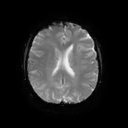
\includegraphics[scale=0.9,angle=0]{Im1.png}
    \caption{IRM sans produit de contraste.}
    \label{fig:without} 
\end{subfigure}
\begin{subfigure}[t]{0.3\textwidth}
\centering
    \vspace{0.00\textheight}
    \includegraphics[scale=0.9,angle=0]{Im7.png}
    \caption{Début de la diffusion.}
    \label{fig:First} 
\end{subfigure}
\begin{subfigure}[t]{0.3\textwidth}
\centering
    \vspace{0.00\textheight}
    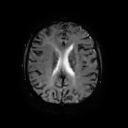
\includegraphics[scale=0.9,angle=0]{Im8.png}
    \caption{Pic de diffusion.}
    \label{fig:Second} 
\end{subfigure}
\begin{subfigure}[t]{0.3\textwidth}
\centering
    \vspace{0.00\textheight}
    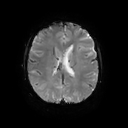
\includegraphics[scale=0.9,angle=0]{Im13.png}
    \caption{Fin de la diffusion.}
    \label{fig:Last} 
\end{subfigure}
    \caption{Diffusion du produit de contraste dans une IRM de perfusion.}
    \label{fig:diffusion} 
\end{figure}

Pour chacune des IRM de cerveau que nous avons récupéré, nous avons donc obtenu un ensemble d'images IRM qui sont réparties selon 24 ou 26 coupes avec pour chaque coupe 40 images traduisant la diffusion du produit de contraste et chaque image est de dimension 256 sur 256 pixels. On a donc pour chaque coupe une tenseur de dimension 256*256*40 qui contient toutes les informations sur la diffusion du produit de contraste.

\medskip

Quelque soit l'IRM considérée, la chaine de traitement restera la même. Il faudra choisir l'IRM d'un patient, stocker les images IRMs par coupe, choisir une coupe puis une région d'intérêt et enfin appliquer l'algorithme sur les éléments sélectionnés comme le montre la figure \ref{fig:toolchain}.


\begin{figure}[H]
\centering
    \includegraphics[scale=0.8,angle=0]{Images/Processing_toolchain.png}
    \caption{Chaine de traitement développée dans le cadre du projet.}
    \label{fig:toolchain}
\end{figure}


La sélection de la région d'intérêt se fait assez facilement avec Matlab comme le montre la figure suivante. L'idée est de prendre une zone et une coupe qui contiennent la zone présentant une pathologie. La partie qui suit va donc consister à expliquer comment on peut, à partir des signaux d'intensité de chacun des pixels, réaliser des clusters qui représentent des tissus homogènes et qui ont donc le même comportement pendant la diffusion du produit de contraste.

\begin{figure}[H]
\centering
    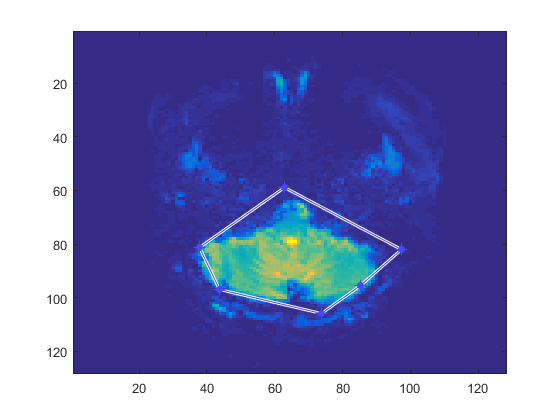
\includegraphics[scale=0.8,angle=0]{Images/ExampleROI.png}
    \caption{Choix d'une région d'intérêt avec Matlab.}
    \label{fig:ExampleROI}
\end{figure}



\chapter{Intérêt de la classification spectrale.}

Il existe une très large bibliographie sur la classification non supervisée. Néanmoins, comme le montre la figure suivante, l'algorithme du K-means ne parvient pas à aboutir au résultat escompté. 

\begin{figure}[H]
\centering
\begin{subfigure}[t]{0.6\textwidth}
\centering
    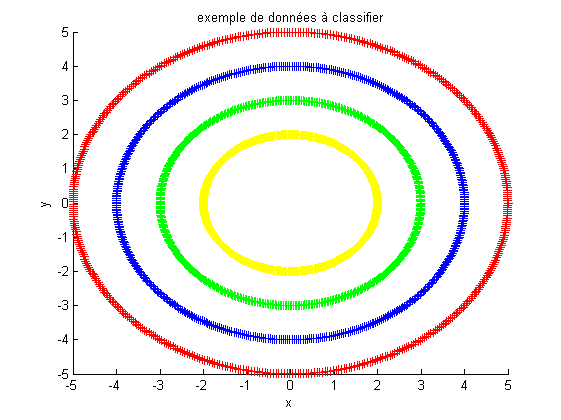
\includegraphics[scale=0.6,angle=0]{Images/DataSet.png}
    \caption{Ensemble de données de départ. Les données sont générées sur un cercle dont le rayon varie selon la classe}
    \label{fig:DataSet}
\end{subfigure}
\begin{subfigure}[t]{0.6\textwidth}
\centering
    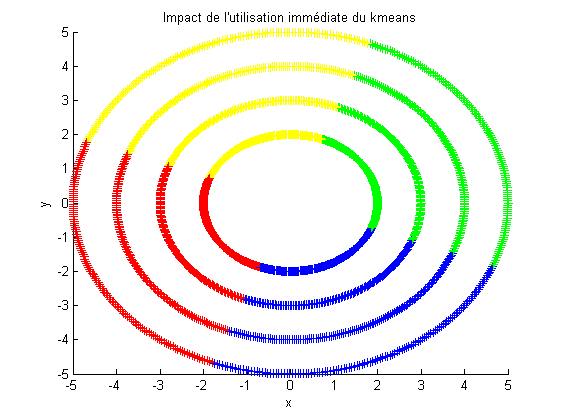
\includegraphics[scale=0.6,angle=0]{Images/AlgoKmeans.png}
    \caption{Application du Kmeans sur cet ensemble de données. Les données ne sont pas correctement classifiées.}
    \label{fig:AlgoKmeans}
\end{subfigure}
\end{figure}

Ici, tous les nuages de points présentent un même centre et cela fausse le résultat bien que des zones de frontières sont facilement identifiable. L'intérêt de la classification spectrale est de construire un graphe par l'intermédiaire d'une matrice de voisinage qui va traduire les similitudes entre les entrées. Ensuite, il faut travailler sur le spectre de cette matrice afin de pouvoir faire une classification. 

\medskip

Dans notre cas d'étude, nous devons étudier des signaux temporels dont on ne connait a priori aucuns paramètres discriminants. Il est donc nécessaire de parvenir à trouver un espace dans lequel la classification puisse aboutir à des résultats pertinents. La classification spectrale est donc ici particulièrement adaptée par rapport au autre algorithme de classification non supervisé.

\chapter{Choix réalisé pour l'implémentation de la classification spectrale.}

Nous devions implémenter un algorithme qui puisse être assez robuste pour traiter différents types d'informations, que ce soit les intensités des pixels des images IRM que nous étudions que des données simulées quelconques. C'est pour cela que certains choix dans la mise en place de l'algorithme ont été fait. Le lecteur pourra trouver en annexe des informations sur la théorie des graphes et également une partie des algorithmes qui ont été développés mais qui n'ont pas servis dans la chaine de traitement finale.

Une fois que l'opérateur a sélectionné une région d'intérêt, on génère une matrice qui contient les courbes d'intensité des pixels sélectionnés. Cette matrice est donnée en entrée de notre chaine de traitement comme le montre la figure \ref{fig:toolchain}.

\section{Choix dans la construction du graphe et de la matrice de similitude.}

Nous voulions avoir une chaine de traitement qui soit la plus robuste et la plus automatisée possible. Nous n'avons aucune connaissance a priori sur les données en entrée donc il faut calculer un coefficient de similitude entre toutes les données entre elles. Par conséquent, on a choisi de construire un graphe entièrement connecté ce qui se traduit par l' attribution d'un coefficient de similitude $W_{ij} = W_{ji}$ pour les signaux du pixel $i$ et du pixel $j$.  

\medskip

On va donc représenter notre graphe par une matrice de similitude W qui aura comme propriété d'être symétrique. Chaque nœud du graphe correspondra à une ligne ou une colonne de la matrice et le coefficient $W_{ij}$ correspondra au lien reliant les nœuds $i$ et $j$. Il faut après définir le coefficient de similitude $W_{ij}$. L'annexe E contient les différentes définitions qui peuvent être choisies. Celle qui donne le plus satisfaction est la similitude euclidienne qui est définie par: 

\medskip


\begin{equation}
W_{ij} = exp(-\frac{d^2(x_i,x_j)}{2\sigma_i\sigma_j})
\end{equation} 

\medskip


Où $x_i$ est le signal du pixel $i$, $\sigma_i$ est un paramètre qui traduit la dispersion des entrées autour de $x_i$ et $d(x_i,x_j)$ est la distance euclidienne entre les signaux $x_i$ et $x_j$. Le document \cite{mouysset2010contributions} donne plusieurs définitions pour ce paramètre et la définition qui donne le plus satisfaction est de prendre $\sigma_i = d(x_i,x_r)$ où $x_r$ correspond au septième voisin le pus proche de $x_i$. 

\medskip


Au final, nous arrivons à une matrice de similitude comme celle ci-dessous pour des données réelles. Cette dernière est affichée en fausse couleur. Les données qui ont été utilisées sont issues d'une IRM de cerveau où on a demandé une classification en 4 classes. La première figure montre la matrice d'affinité une fois tous les calculs réalisés et la seconde montre la matrice d'affinité après l'utilisation de notre algorithme de classification spectrale. On voit nettement 4 blocs au niveau de la diagonal de la matrice. Ces blocs traduisent que les données constitue une classe homogène. Les blocs hors-diagonaux traduisent la ressemblance interclasse. 

\begin{figure}[H]
\centering
    \includegraphics[scale=0.45,angle=0]{Images/MatrixAffinity2.png}
    \caption{Exemple de matrice de similitude.}
    \label{fig:MatrixAffinity2}
\end{figure}


\begin{figure}[H]
\centering
    \includegraphics[scale=0.45,angle=0]{Images/MatrixAffinity.png}
    \caption{Matrice de similitude après utilisation de l'algorithme de classification spectrale.}
    \label{fig:MatrixAffinity}
\end{figure}

Le dernière chose à faire est de définir le laplacien $L$ de la matrice $W$. Pour notre algorithme, nous utilisons le laplacien normalisée symétrique  $L $ défini par:

\begin{equation}
L = I-D^{-1/2}WD^{-1/2}
\end{equation}

Où la matrice $D$, matrice diagonale, contient les degrés des nœuds du graphe. Le degré d'un nœud est défini par $d_i = \Sigma_{v_j \in V} W_{ij}$. Et $I$ est la matrice identité.



\section{Choix de l'algorithme de classification spectrale.}

L'annexe G contient les algorithmes qui ont été implémentés durant le PFE. Pour chacun d'entre eux le principe reste le même. Il faut extraire des informations du spectre de la matrice Laplacienne du graphe qui a été construit avec les remarques ci-dessus. Dans un premier temps, on extrait les plus petites valeurs propres de la matrice L et les vecteurs associés. Ensuite, on applique un algorithme des k-means sur les données générées par la matrice qui contient les précédents vecteurs propres. Il y a plusieurs algorithmes de classification spectrale dans la littérature \cite{mouysset2010contributions} mais l'algorithme de Jordan et Weiss est celui qui nous a donné les meilleurs résultats. Les principales étapes sont données ci-dessous.

\begin{algorithm}[H]
  \caption{Normalized spectral clustering, Jordan and Weiss }
  
  \textbf{Entrées}% Inputs section
  \begin{algorithmic}[1]
    \STATE Matrice $W$ matrice de voisinage
    \STATE Entier $k$ nombre de classe
  \end{algorithmic}
  \bigskip

  \textbf{Sorties}% Output section
  \begin{algorithmic}[1]
    \STATE Vecteur $Ver$ table de vérité calculée.
  \end{algorithmic}
  \bigskip
  
  \textbf{Algorithme}
  \begin{algorithmic}[1]
		\STATE $L\gets$ Laplacien symétrique de la matrice $W$
     	\STATE $VectP\gets$ matrice contenant les vecteurs propres des k plus petites valeurs propres non nulles de L
     	\STATE normaliser toutes les lignes de la matrice $VectP$
     	\STATE $Ver\gets$ résultat de l'algorithme du Kmeans sur la matrice VectP en k clusters.	
  \RETURN $Ver$
  \end{algorithmic}
\end{algorithm}

\section{Choix du nombre de classe.}

Pendant cette étude, plusieurs méthodes ont été implémentées pour trouver automatiquement le nombre optimal de classe en fonction des données d'entrée. Le lecteur trouvera dans l'annexe C quelques algorithmes qui peuvent être utilisés. Sur les données réelles, aucuns d'entre eux ont donné de résultat. Par conséquent, l'opérateur qui utilisera notre algorithme et notre chaine de traitement devra tout de même donner le nombre de classe qu'il souhaite générer. 

\medskip

Au final, notre chaine de traitement a besoin de deux éléments:

\begin{itemize}
\item Une zone d'intérêt ou ROI qui doit être sélectionnée par l'opérateur. Ce qui suppose néanmoins une connaissance a priori sur la zone à étudier.
\item Le nombre de cluster souhaité car il ne peut être trouver de manière automatique.
\end{itemize}

\chapter{Résultats de l'algorithme et interprétations.}


Nous avons dans un premier temps utilisé notre algorithme sur des données simples comme celle qui est utilisé dans le chapitre 5. Voici le résultat que nous obtenons après l'utilisation de l'algorithme que nous avons expliqué dans la partie précédente.

\begin{figure}[H]
\centering
    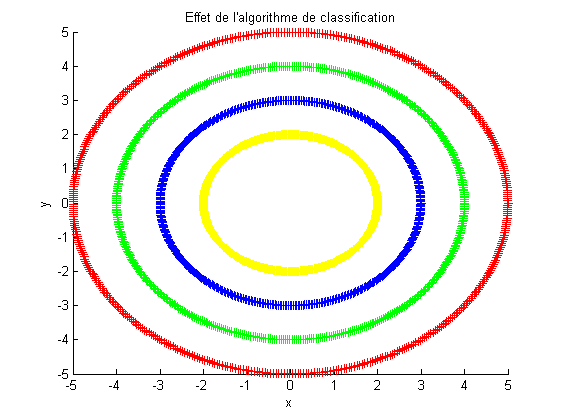
\includegraphics[scale=0.6,angle=0]{Images/AlgoClssification.png}
    \caption{Application du premier algorithme sur les premières données. Les données sont correctement classifiées.}
    \label{fig:AlgoClssification}
\end{figure}

On peut voir que le résultat obtenu est bien celui espéré et que c'est une solution parfaitement viable pour agréger des données dans des clusters bien que les liens entre elles ne soient pas identifiable immédiatement. Les valeurs propres extraites du laplacien et qui sont utilisées pour la classification sont données ci-dessous.

\begin{figure}[H]
\centering
    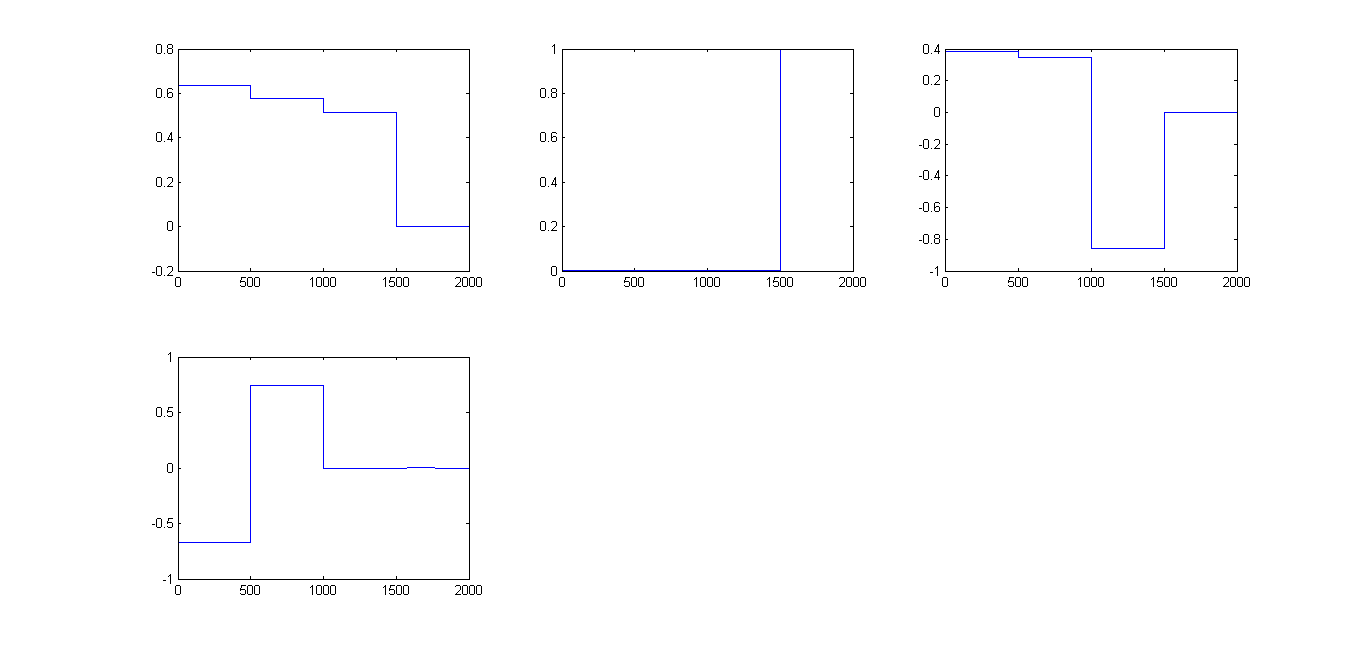
\includegraphics[scale=0.4,angle=0]{Images/VecteursPropres.png}
    \caption{Vecteurs propres extraits du laplacien.}
    \label{fig:VecteursPropres}
\end{figure}

On peut clairement voir comment les K-means, sur ces données extraites, permettent des discriminer les quatre classes. Nous l'avons testé sur un ensemble de test et les figures suivantes montrent les résultats que nous avons obtenu.


\begin{figure}[H]
\centering
    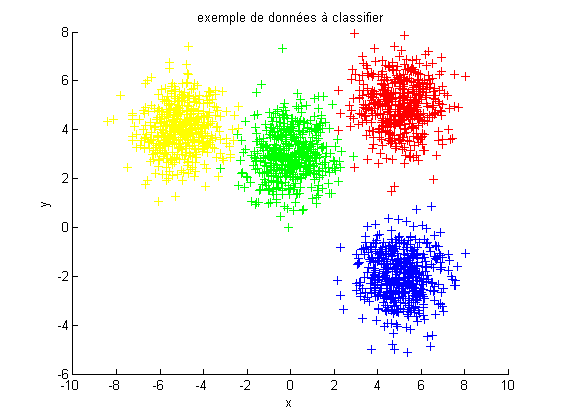
\includegraphics[scale=0.6,angle=0]{Images/DataSet2.png}
    \caption{Second ensemble de données.}
    \label{fig:DataSet2}
\end{figure}

\begin{figure}[H]
\centering
    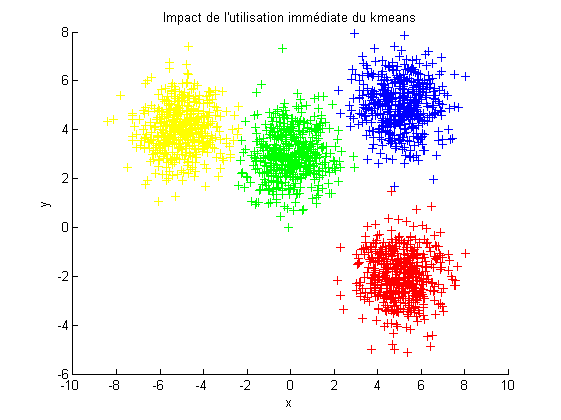
\includegraphics[scale=0.6,angle=0]{Images/AlgoKmeans2.png}
    \caption{Application du Kmeans sur le second ensemble de données.}
    \label{fig:AlgoKmeans2}
\end{figure}

\begin{figure}[H]
\centering
    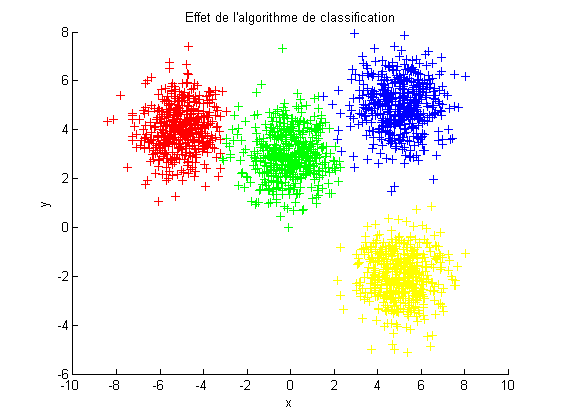
\includegraphics[scale=0.6,angle=0]{Images/AlgoClssification2.png}
    \caption{Application du premier algorithme sur le second ensemble de données.}
    \label{fig:AlgoClssification2}
\end{figure}

\begin{figure}[H]
\centering
    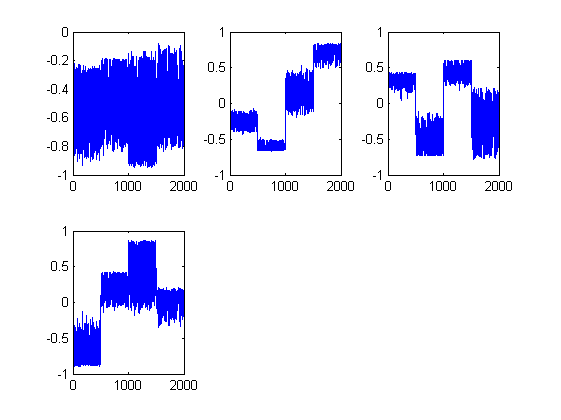
\includegraphics[scale=0.4,angle=0]{Images/VecteursPropres2.png}
    \caption{Vecteurs propres extraits du laplacien.}
    \label{fig:VecteursPropres2}
\end{figure}

Là encore, le résultat est très satisfaisant.


\chapter*{Conclusion}

Au terme de cette étude, nous pouvons extraire ces différents résultats:

\begin{itemize}
\item Tout d'abord, la classification spectrale est particulièrement adaptée pour les problèmes que les algorithmes traditionnels comme le K-means ne peuvent résoudre. On arrive à se placer facilement dans un nouvel espace qui permet d'identifier clairement les éléments appartenant à une même classe. Il est donc tout à fait pertinent pour les signaux que nous devons traiter.
\item La mise en place des différents algorithmes est au final relativement simple et peut couteuse en temps de calcul. Néanmoins, si le nombre de point devient trop grand, il peut y avoir un problème sur le temps d'exécution.
\item La chaine de traitement qui a été développé est très robuste et peut fonctionner dans beaucoup de cas étant donné que nous ne faisons pas d'apriori sur les données de départ et que nous calculons les similitudes de toutes les entrées entre elles.
\end{itemize}

\medskip

Néanmoins, il y a plusieurs contraintes qui faut prendre en compte:

\begin{itemize}
\item Le résultat final est fortement impacté par l'utilisation du K-means à la fin de l'algorithme de classification spectrale. Il arrive que l'algorithme ne converge pas vers les solutions souhaitées en fonction de l'initialisation.
\item Il y a un besoin de connaissance a priori sur le nombre de classe que nous souhaitons. Cela veut dire que notre chaine de traitement ne pourra pas être entièrement autonome.
\end{itemize}



%----------------------------------------------------------------------------------------
%	PART III
%----------------------------------------------------------------------------------------

\part{Résultats.}
\chapter{IMRs T1 de la prostate de l'INSERM de Lille.}

Tous les résultats, codes et bases de données d'images IRM peuvent être trouvés sur le git suivant:

\medskip

https://github.com/chuzelph-ENSTA-Bretagne/ThromboseIRM.git

\medskip

\section{Types de courbe rencontrées dans le cadre du cancer de la prostate}


Le document \cite{doi2007computer} présente les différentes courbes caractéristiques de la prostate. Les courbes d'intensité présentent toutes un hyper signal en IRM T1. Néanmoins, les courbes issus de tissus cancéreux présentent un pic d'absorption beaucoup plus marqué avec un temps d'assimilation très caractéristique alors que les tissus sain présentent une courbe d'absorption beaucoup plus lissée. La figure suivante issue de \cite{doi2007computer} donne une illustration de ces courbes caractéristiques.

\medskip

\begin{figure}[H]
\centering
    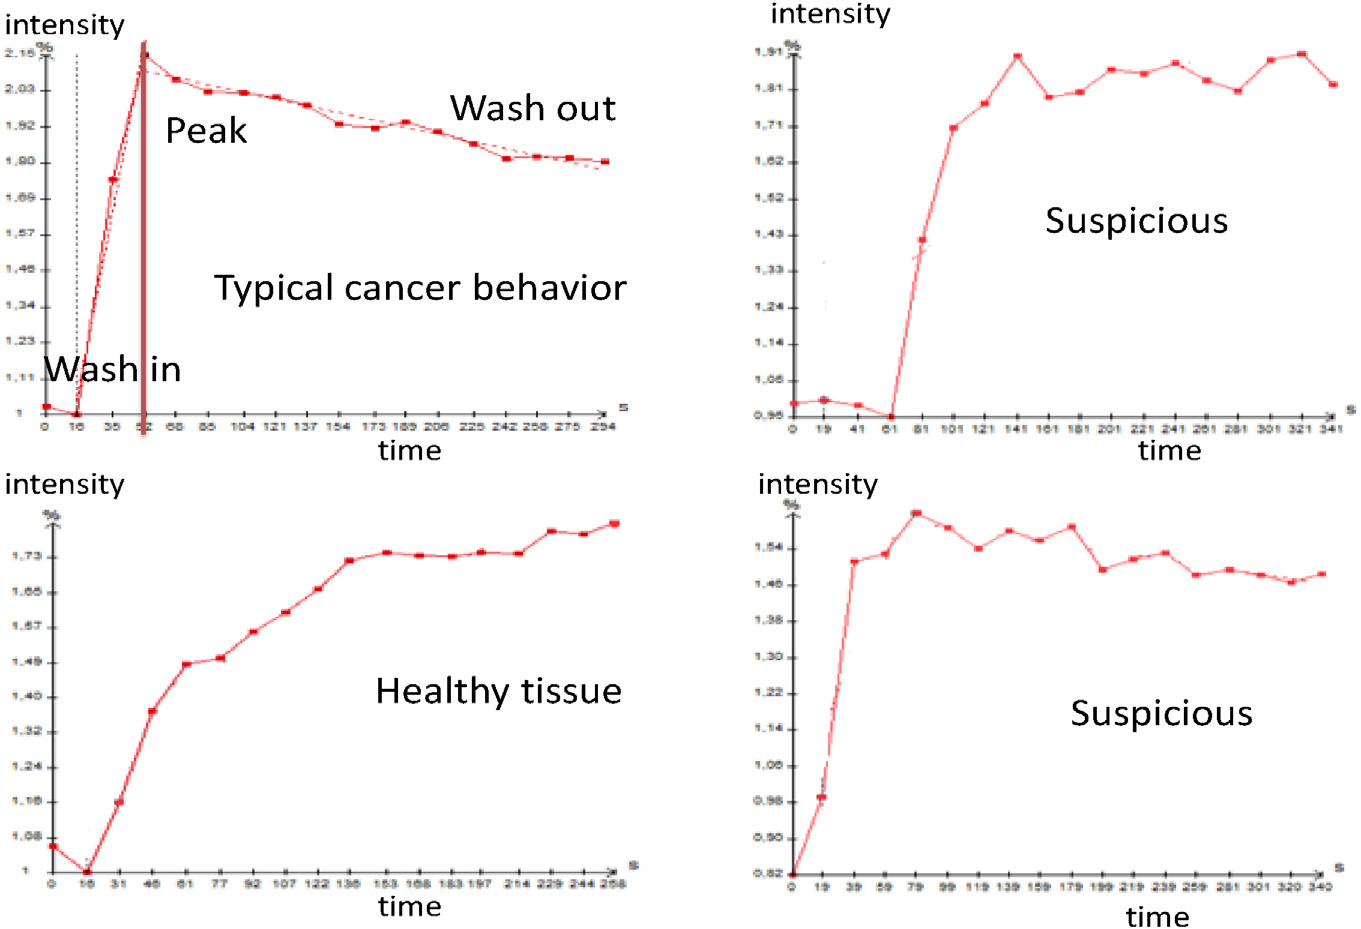
\includegraphics[scale=0.35,angle=0]{Images/CourbeProstate.png}
    \caption{Courbes caractéristiques des tissus sain et cancéreux de la prostate.}
    \label{fig:CourbeProstate}
\end{figure}

\medskip

Néanmoins, certaines courbes sont difficilement à classifier. L'intérêt de notre algorithme va donc être de pouvoir distinguer aisément les tissus sains et les tissus cancéreux et d'estimer avec une autre classe supplémentaire les cas d'incertitude.


\section{Résultats de l'algorithme}

Pour appliquer nos algorithmes, il y a un petit pré-traitement à faire. Pour discriminer les différentes courbes, il faut surtout voir le phénomène de diffusion au sein du tissu et normaliser les courbes afin de faire ressortir le comportement du tissu.
\medskip

Tous les courbes sont donc remise à l'échelle en appliquant la formule suivante:

\begin{equation}
\centering
x(t) \gets \frac{x(t)-x_{min}}{x_{max}-x_{min}}
\end{equation} 

\medskip

Tous les signaux temporels sont donc placés dans une matrice, comme expliqué dans la figure \ref{fig:toolchain}. 
Au final, en appliquant nos algorithmes à une IRM de perfusion de la prostate, nous arrivons au résultat suivant :

\begin{figure}[H]
\centering
    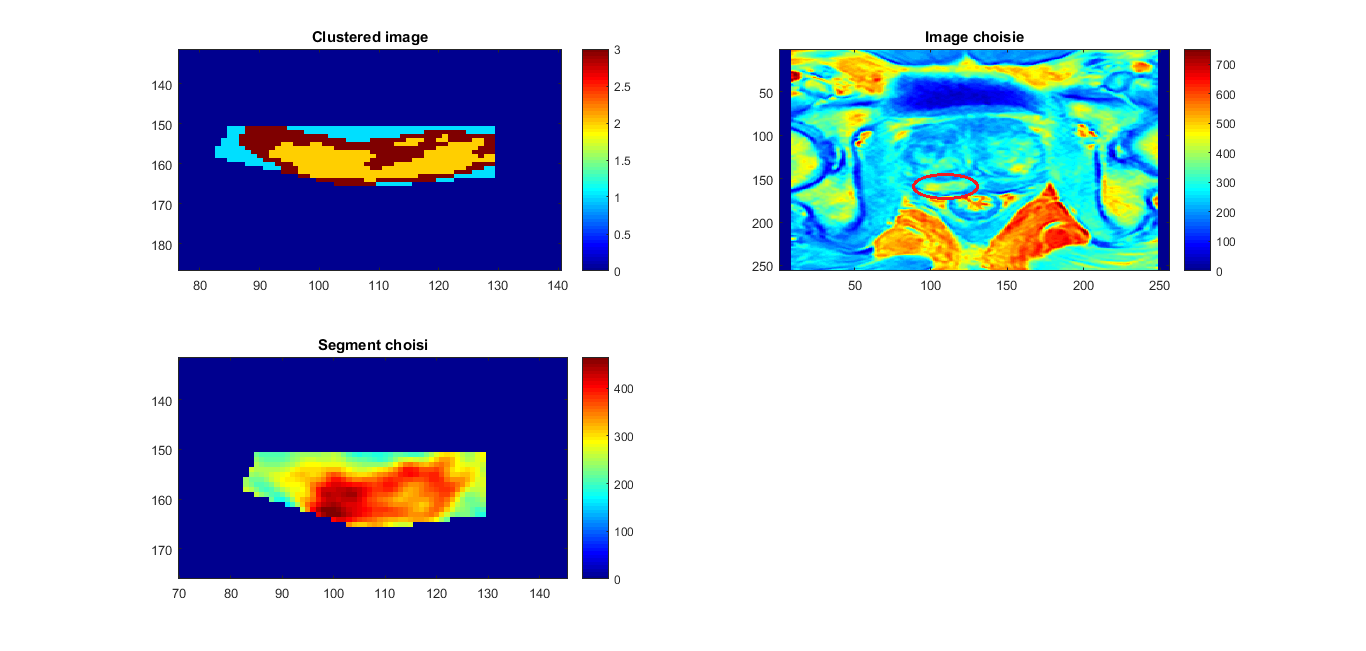
\includegraphics[scale=0.4,angle=0]{Images/3classProstate2.png}
    \caption{Coupes sélectionnées. En haut à gauche le résultat de l'algorithme de classification. En haut à droit, image de la coupe sélectionnée avec la ROI représentée par l'ellipse rouge. En bas à gauche, ROI en fausses couleurs.}
    \label{fig:3classProstate2}
\end{figure} 

La figure suivante montre comment les courbes sont réparties selon les différents clusters.

\begin{figure}[H]
\centering
    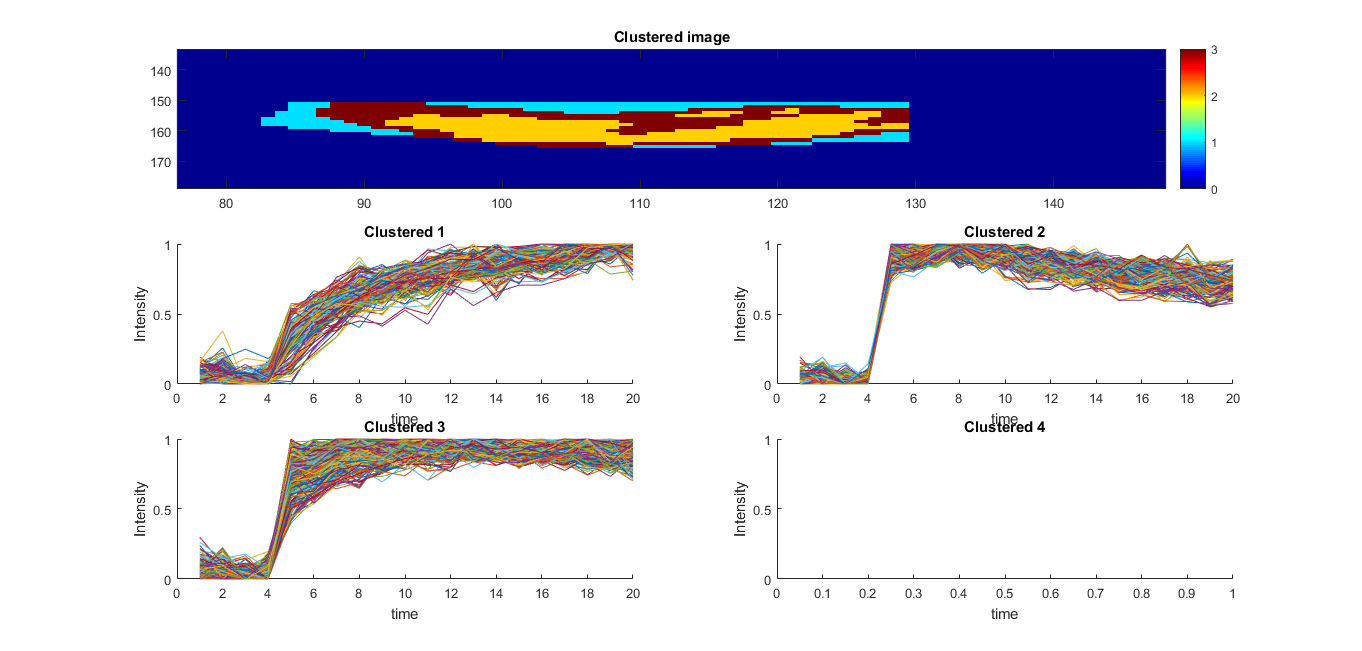
\includegraphics[scale=0.4,angle=0]{Images/3classProstate.png}
    \caption{Résultat de l'algorithme sur l'IRM avec les courbes associées aux clusters.}
    \label{fig:3classProstate}
\end{figure}

Nous avons ici lancé une simulation avec 3 classes. Nous pouvons interpréter ces résultats de la façon suivante:

\begin{itemize}
\item Le cluster 1 rassemble les courbes qui sont saines en accord avec les informations issus de la figure \ref{fig:CourbeProstate},
\item Le cluster 2 lui rassemble les courbes des tissus tumoraux qui présentent un temps d'absorption très court et un pic très marqué,
\item Le cluster 3 lui représentent des courbes qui sont suspectes. Ici, l'algorithme comme l'humain va avoir du mal à trancher sur l'appartenance de ces tissus au sain ou tumoral.
\end{itemize}

Le résultat obtenu est très satisfaisant et on arrive à un résultat semblable à ceux obtenus dans \cite{doi2007computer} bien que la chaine de traitement ne soit pas la même. 

Néanmoins, il y a quelques remarques à faire:

\begin{itemize}
\item Il faut parfois choisir une bonne représentation des données de départ afin que l'algorithme converge vers une solution satisfaisante.
\item Il est nécessaire de choisir une ROI qui est composée d'une zone de taille pas trop importante. En effet, l'algorithme ne converge pas si il y a trop de points sélectionnés.
\end{itemize}


\chapter{IMRs T2 du crane CHRU Brest Cavale Blanche.}

Le CHRU de Brest nous a permis de constituer un base de données de 13 patients présentant des lésions cérébrales caractéristiques sur lesquels nous avons pu tester notre chaine de traitement. Les deux exemples qui vont être présentés ici sont particulièrement pertinents sur les capacités et limites de la méthode pour cette partie du corps. Les IRM que nous utilisons ici sont des IRM T2 ce qui implique que nous aurons la présence d'un hypo-signal pendant la diffusion du produit de contraste.

% Figure avec IRM en niveau de gris de la tumeur
\begin{figure}[H]
\centering
    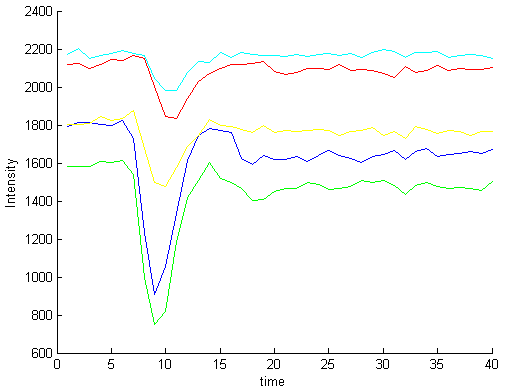
\includegraphics[scale=0.8,angle=0]{Images/CourbeExample.png}
    \caption{Exemples de courbes obtenues par les IRM du CHRU.}
    \label{fig:CourbeExample}
\end{figure}

Nous pouvons créer deux cartes paramétriques à partir des IRM de perfusion qui peuvent aider pour faire un diagnostic. Le premier paramètre est le CBV ou \textit{cerebral brain volume}. Ce paramètre permet de traduire l'importance d'absorption de produit de contraste par le tissu considéré. Le document \cite{muir2014quantitative} définit le CBV par la méthodologie suivante. Le temps de relaxation transversal $\Delta R2^*$ est donné par la formule:

\begin{equation}
\Delta R2^*(t) = \frac{-ln(S(t)/S_0}{TE}
\end{equation}

où $TE$ est le temps de pulsation d'écho de l'IRM. Il est récupérable sur les méta-données de l'IRM. Le CBV est donc défini comme l'intégrale de $R2^*(t)$

\begin{equation}
CBV = \int^{t_f}_{t_0} R2^*(t) dt
\end{equation}

Le second paramètre est le CBF ou \textit{cerebral brain flow}. Il n'est pas pertinent pour l'étude que nous avons menée mais il a été implémenté sur Matlab.

\medskip



\section{Patient 1: Cancer identifiable par l'IRM de perfusion.}

L'IRM qui est ici présentée provient d'un patient qui a un cancer bénin situé à la frontière du cerveau et de la boite crânienne. La tumeur est visible sur la figure suivante à sur la partie gauche de l'image. A sa droite, on peut voir la présence d'un assez gros œdème résultant de la présence de la tumeur. Le reste du cerveau est sain et il y a au centre de l'image le ventricule cérébrale qui produit le liquide céphalo-rachidien. Ce dernier apparait ici avec un hyper-signal caractéristique.

% Figure avec IRM en niveau de gris de la tumeur
\begin{figure}[H]
\centering
    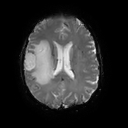
\includegraphics[scale=2,angle=0]{Images/Patient4IRM.png}
    \caption{IRM du patient présent une tumeur bénigne et un œdème.}
    \label{fig:patient4IRM}
\end{figure}

Nous avons donc appliqué notre algorithme en sélectionnant une ROI qui ne contient pas le ventricule cérébral afin qu'il ne vienne pas parasité le résultat de l'algorithme. Nous avons également demandé qu'il ressorte quatre classes. La figure qui suit montre dans l'ordre, l'IRM du patient en fausse couleur, la carte paramétrique du CBV et le résultat de notre algorithme.

% Figure du patient 4 avec les résultats du programme.
\begin{figure}[H]
\centering
    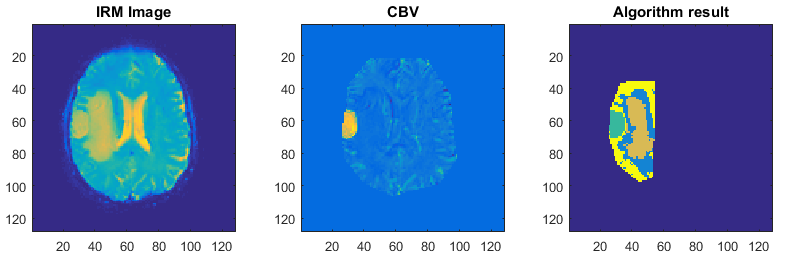
\includegraphics[scale=0.8,angle=0]{Images/Patient4Result.png}
    \caption{Résultat de l'algorithme.}
    \label{fig:patient4IRMResult}
\end{figure}

La carte de CBV est ici particulièrement adaptée car elle fait ressortir tout tissu qui a tendance à absorber un grand volume de produit de contraste par rapport au reste du cerveau. Sur cette carte, on voit que la tumeur est immédiatement isolée.

On peut remarquer que l'algorithme que nous avons mis en place permet d'isoler parfaitement la tumeur mais également l'œdème et permet d'établir une zone de frontière entre cette œdème et les tissus sains.

\bigskip
\begin{Large}
\textcolor{blue}{Conclusion:}
\end{Large}
\medskip

On peut voir par cette exemple que notre algorithme est particulièrement adapté pour cette pathologie car cette tumeur impacte beaucoup la diffusion du produit de contraste. Néanmoins, on peut regretter que nous ne pouvons détecter que un unique œdème avec notre algorithme.


\section{Patient 2: Cancer non-identifiable par l'IRM de perfusion.}

L'IRM qui suit provient d'un patient qui a un cancer situé dans la région en haut à gauche du cerveau. On peut voir un très gros œdème qui est situé tout autour de la tumeur mais cette dernière n'implique pas de modification notable de la diffusion du produit de contraste ce qui se traduit par un CBV qui n'est pas particulièrement modifié.

% Figure avec IRM en niveau de gris de la tumeur
\begin{figure}[H]
\centering
    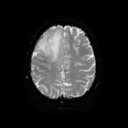
\includegraphics[scale=2,angle=0]{Images/Patient2IRM.png}
    \caption{IRM du patient présent une tumeur et un œdème. Ici, seul l'œdème est identifié par notre algorithme.}
    \label{fig:patient4IRM}
\end{figure}

\begin{figure}[H]
\centering
    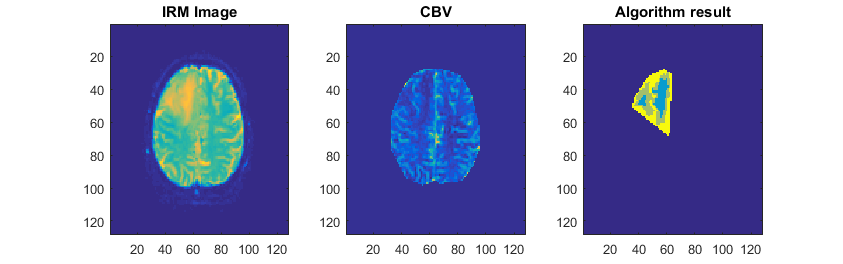
\includegraphics[scale=0.8,angle=0]{Images/Patient2Result.png}
    \caption{Résultat de l'algorithme.}
    \label{fig:patient4IRMResult}
\end{figure}

Nous avons testé notre algorithme en demandant la création de 2 et 3 classes et on retrouve un résultat similaire à celui ci-dessus. On observe que dans le cas où on demande deux classes, on a l'œdème qui est identifié et pour 3 classes, on a une zone frontière qui se créer entre le tissu sain et l'œdème. Néanmoins, la tumeur ne peut être identifier.

\begin{figure}[H]
\centering
\begin{subfigure}{.5\textwidth}
    \centering
    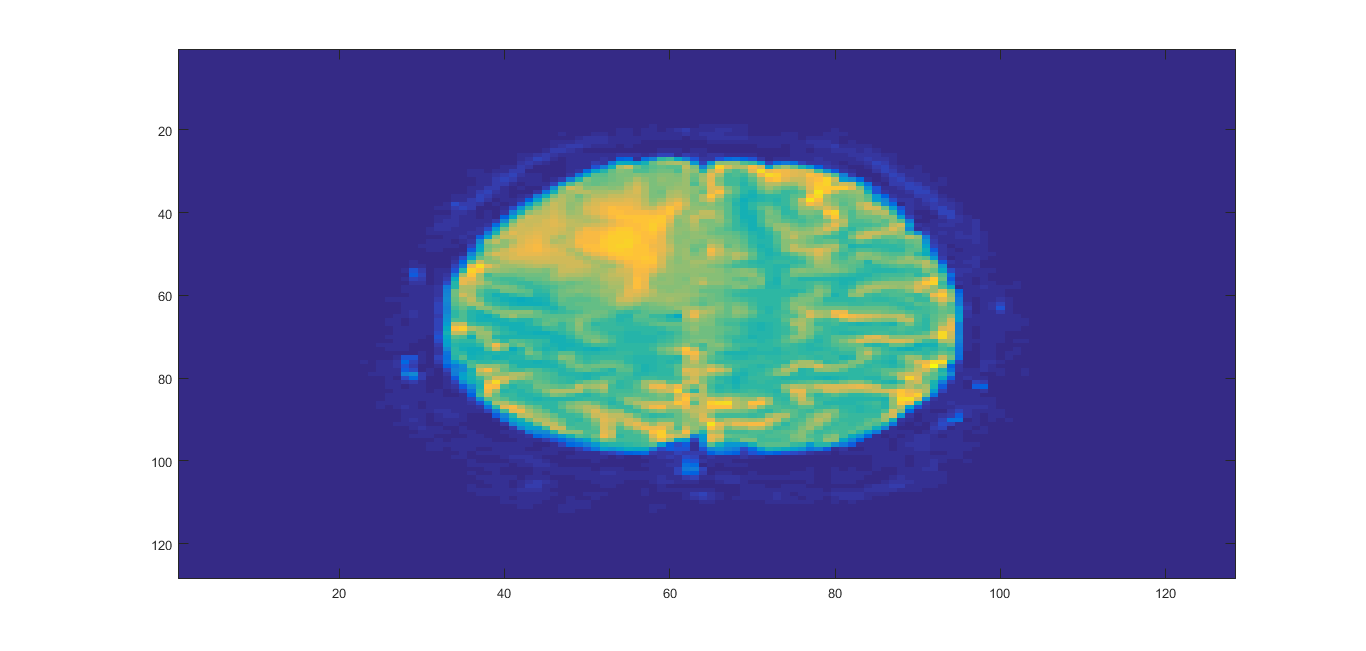
\includegraphics[scale=0.2,angle=0]{Images/TrueclassBrain.png}
    \caption{Image originale.}
    \label{fig:TrueclassBrain} 
\end{subfigure}
\begin{subfigure}{.33\textwidth}
    \centering
    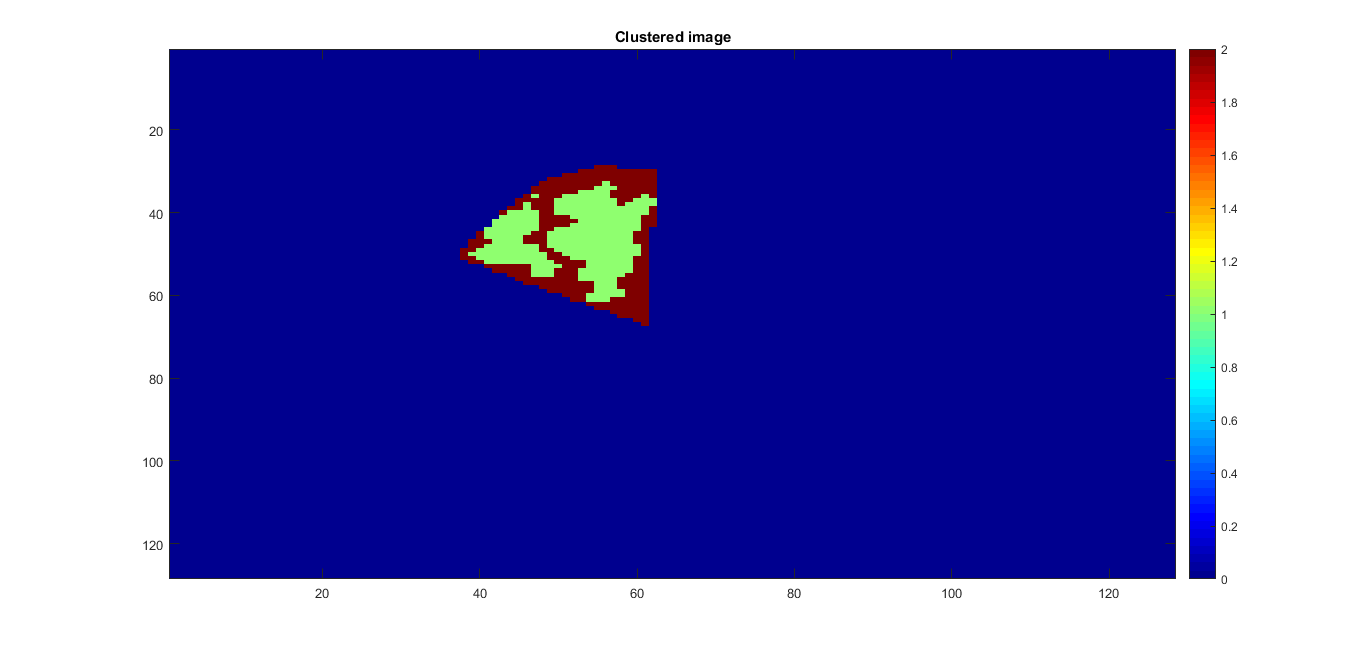
\includegraphics[scale=0.2,angle=0]{Images/2classBrain.png}
    \caption{Résultat de l'algorithme avec 2 classes.}
    \label{fig:2classBrain} 
\end{subfigure}
\begin{subfigure}{.33\textwidth}
    \centering
    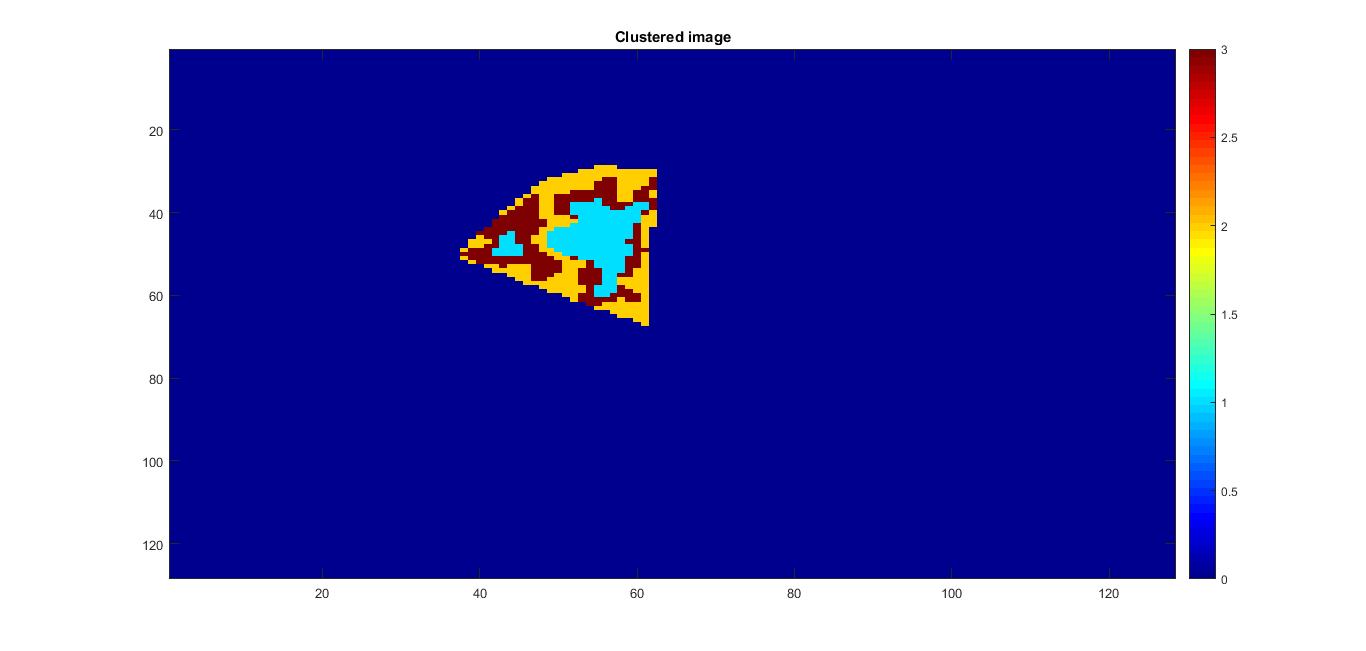
\includegraphics[scale=0.2,angle=0]{Images/3classBrain.png}
    \caption{Résultat de l'algorithme avec 3 classes.}
    \label{fig:3classBrain} 
\end{subfigure}
    \caption{Résultats de notre algorithme sur le patient 2 avec 2 et 3 classes.}
    \label{fig:2and3classBrain} 
\end{figure}

\bigskip
\begin{Large}
\textcolor{blue}{Conclusion:}
\end{Large}
\medskip


Tant notre algorithme que la carte de CBV sont ici inadapté pour cette pathologie. Bien que on identifie clairement l'œdème, le principal but de notre algorithme est de pouvoir identifier des pathologies plus graves comme les tumeurs. Mais dans certains cas comme celui ci-dessus, il est nécessaire de trouver d'autres sources d'information plus pertinentes pour proposer une segmentation de la zone pathologique.


\part*{Conclusion}
Ce stage m'a permis de me former sur beaucoup de problématiques en rapport avec le milieu médical et rencontrer plusieurs médecins qui m'ont appuyé. Cela m'a demandé de développer un esprit d'initiative afin de voir et résoudre les problèmes qui sont présentés devant moi durant ces 6 mois. J'ai pu approfondir mes connaissances sur des domaines scientifiques comme la classification non supervisée et j'ai pu voir comment il faut analyser des images médicales. Ce stage fut très intéressant et épanouissant.

\medskip

L'objectif que nous nous sommes fixé au départ était de réaliser un programme d'aide au diagnostic pour les pathologies cérébrales. Au final, la chaine de traitement que nous avons mis en place présente plusieurs caractéristiques:

\begin{itemize}
\item elle est très fortement automatisée. L'opérateur qui souhaiterait l'utiliser n'aura qu'à sélectionner une zone d'intérêt suspecte sur l'image IRM et le nombre de tissu qu'il semble voir à l'image.
\item Pour certaines pathologies, l'algorithme développé permet d'isoler la pathologie de la zone présentant des tissus sains.
\item Néanmoins, pour d'autres pathologies, les IRM de perfusion que nous avons utilisé ici ne permettent pas d'aboutir à un résultat.
\end{itemize} 

L'objectif que l'on m'a posé est donc partiellement atteint. Ce résultat est intéressant mais une piste semble prometteuse pour résoudre ce problème . Nous nous sommes ici principalement focalisés sur l'étude d'un seul type d'IRM alors que les médecins se servent de plusieurs modalités d'image IRM pour faire leur diagnostic. L'analyse multimodale semble donc tout indiquée cependant le temps imparti ne m'a pas permis d'implémenter cette solution.



\appendix
\part{Annexes}
\chapter{Anonymisation des images DICOM}

Pour anonymiser les données, j'utilise le programme "Santé Dicom Editor". Il suffit d'ouvrir le dossier contenant les images et aller dans l'onglet Edit $\rightarrow$ Anonymise current file/series. Il existe des fonctions Matlab pour faire le même travail mais certains champs sensibles étaient malgré tous intacts. Voir \textit{http://www.santesoft.com/win/sante\_ dicom\_ editor/sante\_ dicom\_ editor.html}.

\begin{figure}[H]
\centering
    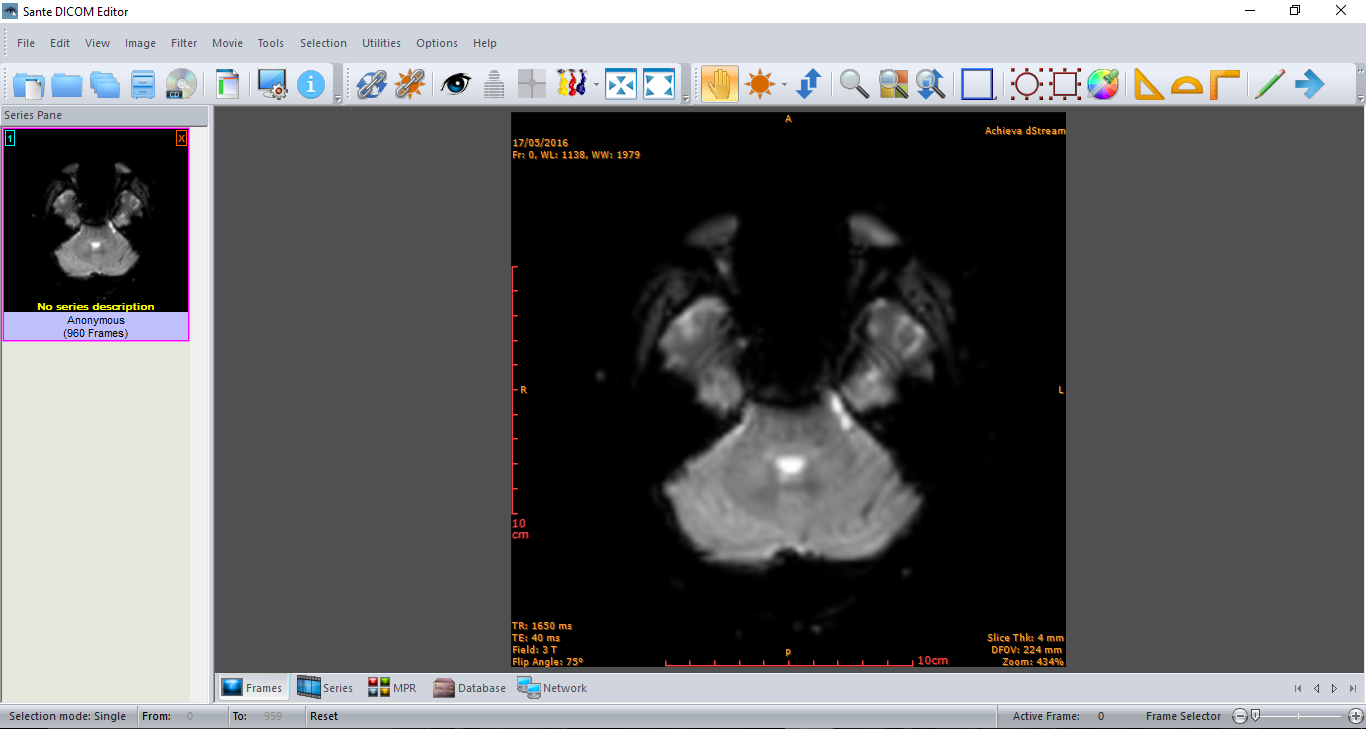
\includegraphics[scale=0.35,angle=90]{Images/AnonExe.png}
    \caption{Programme pour l'anonymisation des données.}
    \label{fig:AnonExe}
\end{figure}

\chapter{Visualisation des données en 3D et 4D}

Un gros problème lorsque nous recevons les images Dicom est que nous ne pouvons voir de façon très claire la localisation de la tumeur. J'ai donc réutilisé et modifié des codes Matlab disponibles sur internet afin d'avoir une représentation 3D et 4D. Ils sont disponibles sur les liens suivant:

\medskip

\textit{http://fr.mathworks.com/matlabcentral/fileexchange/41465-4d-volume-visualization}

\textit{http://www.mathworks.com/matlabcentral/fileexchange/37268-3d-volume-visualization}



\begin{figure}[H]
\centering
    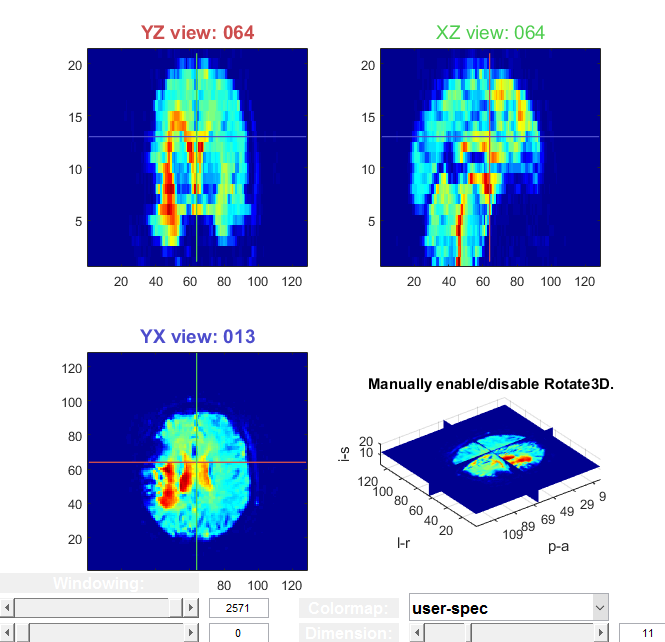
\includegraphics[scale=0.8,angle=0]{Images/4D.png}
    \caption{Programme Matlab pour la visualisation de données en 4D.}
    \label{fig:4D}
\end{figure}

\chapter{Choix automatique du nombre de classe.}

\section*{Algorithme 1 : Analyse des valeurs propres et le n-gap}

Dans le cas d'une classification idéale, la matrice laplacienne $L$ peut être mise sous la d'une matrice par bloc où tout les blocs non-diagonaux sont nuls.

\medskip

$
L = 
\begin{bmatrix}
   x^{(1)} &0 &\cdots &0 \\
   0 &x^{(2)} &\ddots &\vdots\\
   \vdots &\ddots &\ddots &0\\
   0 &\cdots &0 &x^{(n)}
\end{bmatrix}
$

\medskip

Cela traduit le fait que les blocs ou clusters sont homogènes et ne présentent pas de similitude entre eux. Cependant, vu comment la matrice L est construite, la valeur propre 0 va avoir une multiplicité égale au nombre de bloc.

\medskip

Une première méthode consiste donc à afficher les $n$ premières valeurs propres de L et de "compter" le nombre de fois que la valeur propre 0 apparait. Dans le cas des données simulées ci-dessous:

\medskip

\begin{figure}[H]
\centering
    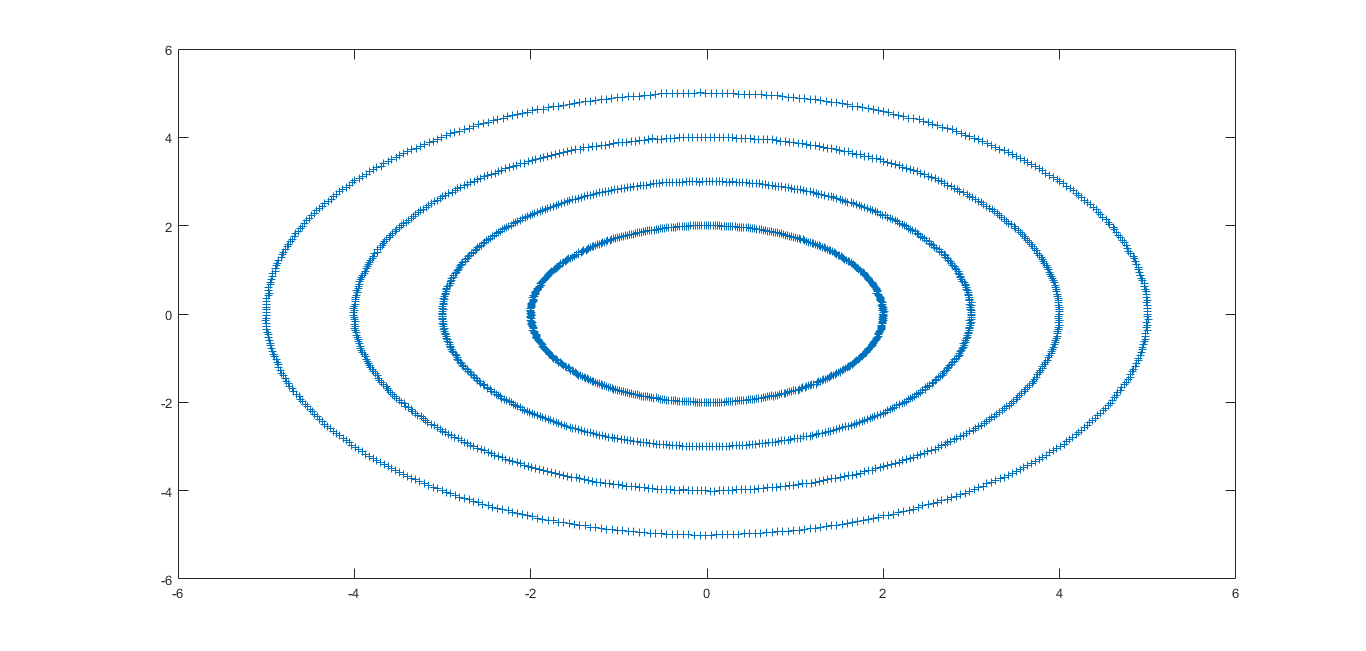
\includegraphics[scale=0.4,angle=0]{Images/testData.png}
    \caption{Exemple simple de données à classifier. Le nombre de classe est 4.}
    \label{fig:testData}
\end{figure} 

\medskip

Nous arrivons au valeurs propres suivantes:

\medskip

\begin{figure}[H]
\centering
    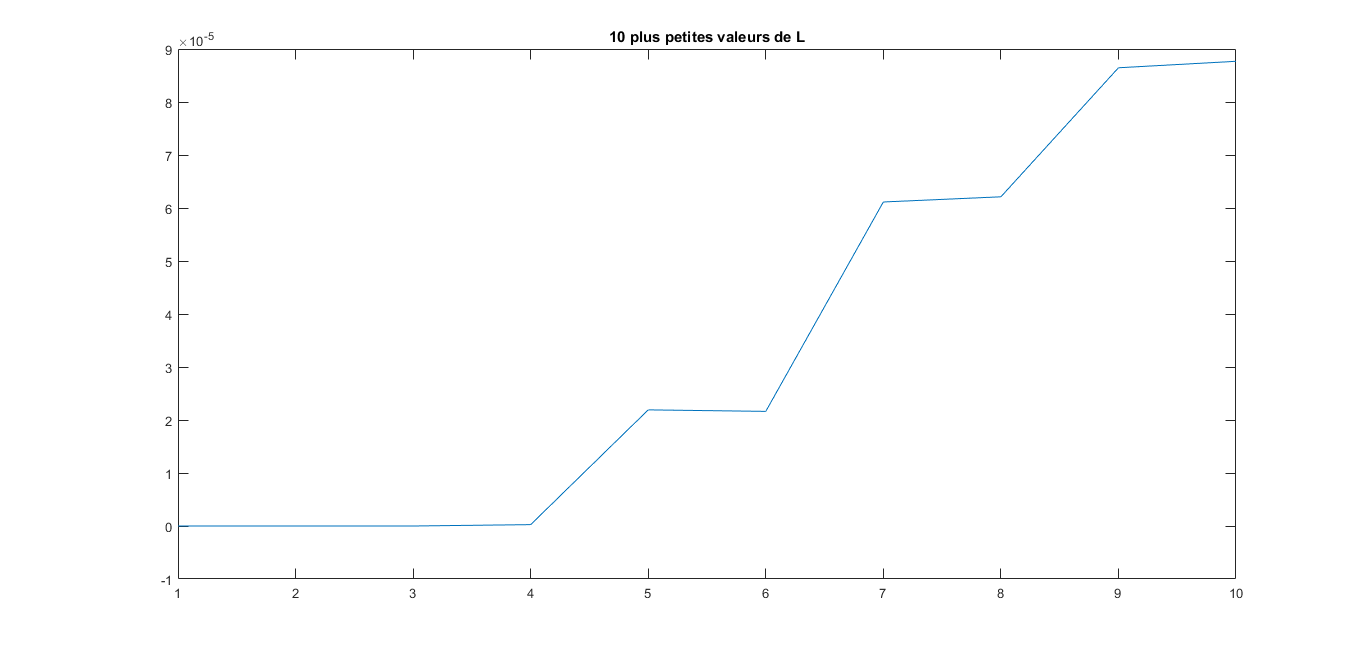
\includegraphics[scale=0.4,angle=0]{Images/Ngap.png}
    \caption{10 plus petites valeurs propres de L. On observe bien que on a un saut à partir de n=5. Le nombre optimal de classe est 4.}
    \label{fig:Ngap}
\end{figure} 

\medskip

Une autre méthode consiste à calculer la différence entre deux valeurs propres successives et voir à partir de quand un gap significatif se produit afin d'identifier le nombre de classe optimale. Néanmoins, ces deux méthodes sont hautement discutables de par leur manque de rigueur.


\section*{Algorithme 2 : Minimisation par la norme de Frobenius}

Une autre méthode consiste à voir pour quel nombre de classe la similitude entre classe est la plus faible.
On définit la norme de Frobenius d'une matrice par la formule suivante:

\medskip
$
\|{L}\|_F = \sum_{i=1}^{N_i}  \sum_{j=1}^{N_j} |L_{ij}|
$
\medskip

L'idée va donc être de calculer le volume des blocs diagonaux et de calculer une fonction coût qui dépend du nombre de classe.

\begin{figure}[H]
\centering
    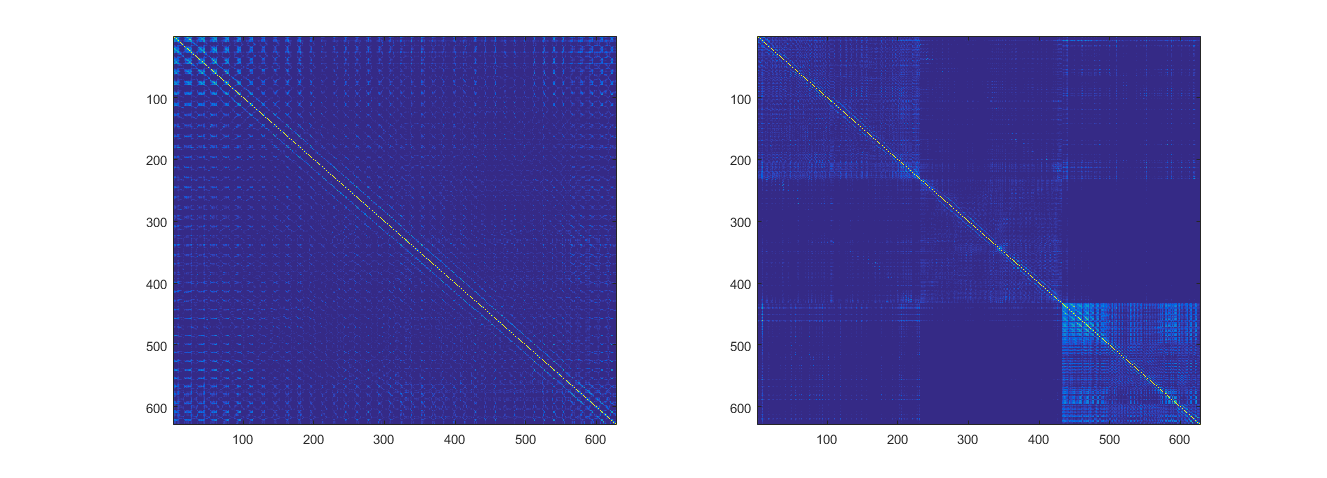
\includegraphics[scale=0.4,angle=0]{Images/L.png}
    \caption{Exemple de matrice laplacienne avant et après utilisation de l'algorithme de classification spectrale en trois classes et ré-agencement. On observe bien l'apparition de blocs.}
    \label{fig:L}
\end{figure} 

On définit donc le ratio de Frobenius entre deux blocs de la matrice L par:

\medskip

$
r_{ij} = \frac{ \|{L^{ij}}\|_F }{\| L^{ii} \|_F}
$

\medskip

On va donc regarder les valeurs de $r_{ij}$ et voir pour quel valeur de $n$ on atteint un minimum. Le but de cet algorithme va consister à trouver la valeur de $n$ qui va minimiser la fonction :

\medskip

$
\nu_k = \frac{2}{k(k-1)}\sum_{i=1 , j=i+1}^{k}(r_{ij})
$

\medskip

Il faut donc regarder pour plusieurs valeurs de n quel est le nombre de classe qui minimise cette fonction.

\section*{Application de ces algorithmes sur des données réelles.}

Sur des données simulées, les algorithmes précédents donnent de bons résultats mais cela n'est absolument pas le cas pour les données issues des IRM de cerveau. Les algorithmes ne semblent pas capables de déterminer de façon claire un nombre de classe optimal pour les signaux.

\chapter{Réalisation de programme pour le milieu médical en stand-alone.}

La société MathWorks propose un outil pour la réalisation de programme utilisant directement les fichiers Matlab. A partir d'une interface qui peut être très facilement crée par l'outil GUIDE de Matlab, on peut assez facilement proposer un programme qui peut être installé sur tout ordinateur ayant Windows comme système d'exploitation. 

\begin{figure}[H]
\centering
    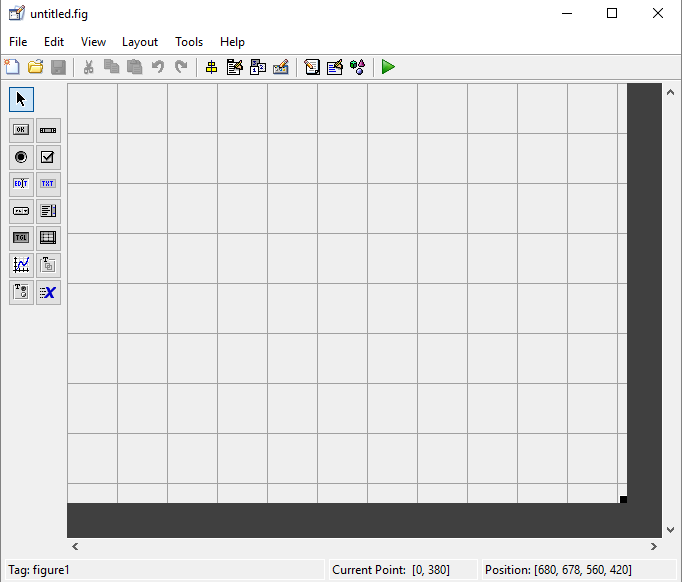
\includegraphics[scale=0.4,angle=0]{Images/Guide.png}
    \caption{Présentation de l'outil de Guide de Matlab.}
    \label{fig:Guide}
\end{figure} 

\begin{figure}[H]
\centering
    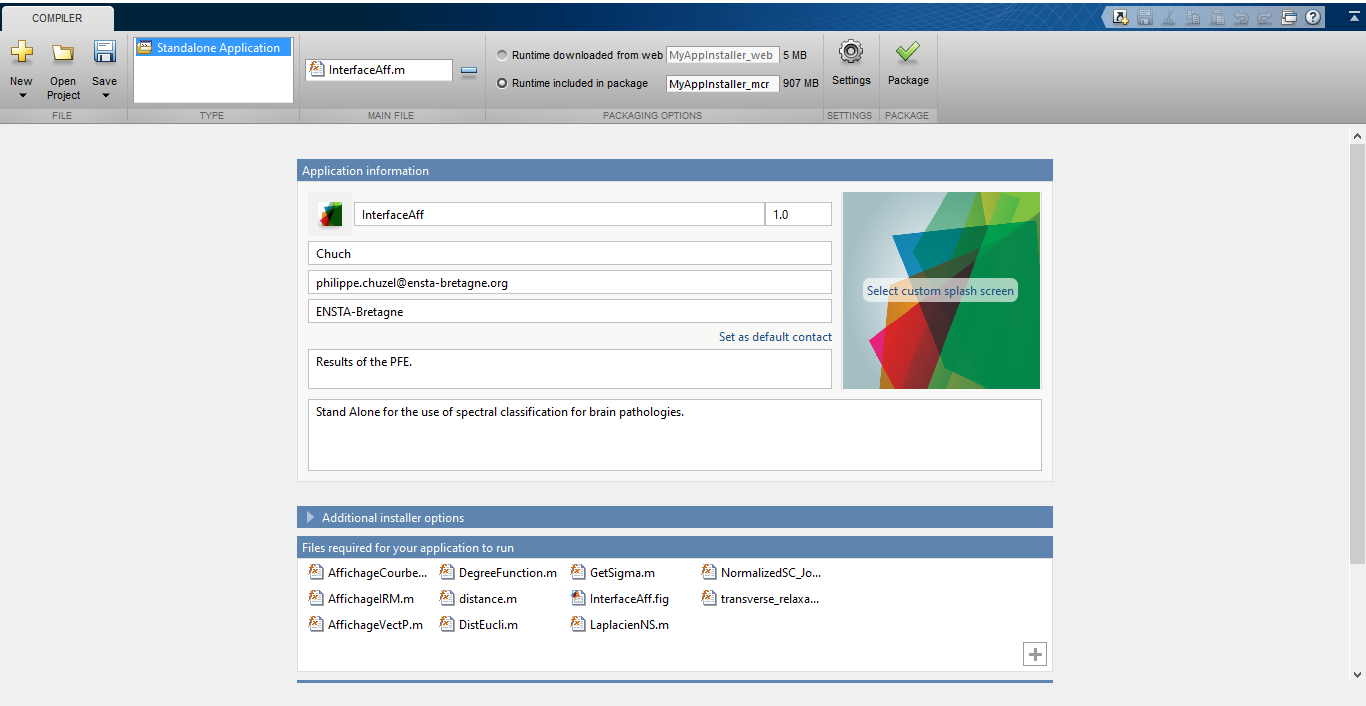
\includegraphics[scale=0.4,angle=0]{Images/StandAlone.png}
    \caption{Présentation de l'outil de Application Compiler de Matlab.}
    \label{fig:Compiler}
\end{figure} 

Néanmoins, l'exécutable qui est généré est très lourd, autour de 1GB ce qui est assez contraignant. Ce sont surtout les dépendance avec les bibliothèques en C et C++ qui impose un tel volume.

La meilleur solution si nous souhaitons avoir un programme entièrement portable est donc de passer le code en C++ et de réaliser une interface avec une bibliothèque adaptée du type QT.

\chapter{Rappel sur la théorie des graphes.}

\section{Définitions de base.}

Un graphe est constitué du couple (V,E,W), où V correspond à ensemble des nœuds du graphe, E correspond à l'ensemble des couple $(v_i,v_j)$ symbolisant le lien entre deux nœuds et W correspond à la matrice de voisinage. Par définition, le coefficient $W_{ij}$ prend comme valeur le poids liant le nœud $v_i$ au nœud $v_j$. Il s'en suit que la matrice W est symétrique. Nous verrons plus tard comment nous pouvons construire une tel matrice.


Par la suite, nous définissons la matrice D, diagonale, qui contient les degrés des nœuds du graphe. Le degré d'un nœud est défini par $d_i = \Sigma_{v_j \in V} W_{ij}$. 
\section{Choix du laplacien de la matrice.}

Il existe trois définition différentes de laplacien d'une matrice. Si on appelle $D$ la matrice de degré du graphe et $W$ la matrice de voisinage du graphe, on aboutie aux définitions suivantes.

\paragraph{Matrice Laplacienne standard non normalisée}

\medskip 

Ce laplacien est donné par la relation:

\begin{equation}
L = D-W
\end{equation}


\paragraph{Matrice Laplacienne normalisée asymétrique}

\medskip 

Ce laplacien est donné par la relation:

\begin{equation}
L = I-D^{-1}W
\end{equation}


\paragraph{Matrice Laplacienne normalisée symétrique}

\medskip 

Ce laplacien est donné par la relation:

\begin{equation}
L = I-D^{-1/2}WD^{-1/2}
\end{equation}

Ces trois matrices présentent les mêmes propriétés:

\begin{itemize}
\item Ces matrices présentent la valeur propres 0 une seule fois pour le vecteur propre $I$ ou $D^{1/2}I$.
\item Ces matrices sont réelles semi-définies positives.
\end{itemize}

Par conséquent, quand nous chercherons à trouver les k plus petites valeurs propres de cette matrice, il nous sera possible très facilement de les récupérer.

\chapter{Construction de la matrice de voisinage.}


Il y a trois choix à faire pour définir la matrice de voisinage d'un graphe.

\section{Choix du type de voisinage.}

Pour un ensemble de nœud donné, il y a plusieurs manière de créer les liens qui vont compléter l'ensemble (E,V,W).

\medskip

\textbf{Graphe des epsilons voisin}: On considère ici que deux nœuds ont un lien si la distance entre eux est inférieur à $\epsilon$.

\medskip

\textbf{Graphe des k-plus proche voisins}: On considère ici que tous les nœuds ont k voisins et qu'ils sont les k-plus proche du nœud considéré.

\medskip

\textbf{Graphe entièrement connecté}: On considère que tous les sommets sont reliés entre eux. 

\medskip

Ici, nous avons implémenté le graphe entièrement connecté car il nous donne de très bons résultats et qu'il est très simple à mettre en place.

\section{Choix de la distance et de la similitude.}

Dans la littérature de la classification, il est nécessaire de choisir une distance et une fonction de similarité.

\medskip

Plusieurs choix s'offre à nous pour les distances:

\begin{itemize}

\medskip

\item \textbf{Distance de Manhattan} : $\Sigma_i|x_i-y_i|$

\medskip

\item \textbf{Distance d'euclidienne} : $(\Sigma_i(x_i-y_i)^2)^(1/2)$

\medskip

\item \textbf{Distance de Minkowski} : $(\Sigma_i|x_i-y_i|^p)^(1/p)$

\medskip

\end{itemize}

La distance euclidienne a ici été choisie.

\medskip

La fonction de similitude doit être une fonction qui va associer une valeur comprise entre 0 et 1 à deux sommet du graphe:

\begin{equation}
f(x_i,x_j) \Rightarrow [0 ; 1]
\end{equation}

La littérature donne plusieurs types de fonction de similitude mais deux sont à retenir.
\begin{itemize}

\item La similitude euclidienne qui est définie par la fonction \\
\begin{equation}
f(x_i,x_j) = \frac{1}{1+\frac{d^2(x_i,x_j)}{\sigma^2}}
\end{equation}

\item La similitude gaussienne qui est définie par la fonction \\
\begin{equation}
f(x_i,x_j) = exp(-\frac{d^2(x_i,x_j)}{2\sigma^2})
\end{equation}

\end{itemize}


Dans les deux cas, le coefficient $\sigma$ est un paramètre qui traduit la dispersion des données. Nous avons ici choisi la similitude gaussienne car elle permet de traduire de manière plus efficace la similitude des données.
 
\section{Choix du paramètre de dispersion.}

Le gros problème pour les données que nous aurons à traiter est que le paramètre $\sigma$ devra être déterminé de manière automatique en fonction des données d'entrées.Ce paramètre va traduire la similitude ou non des différents éléments entre eux et donc va conditionner tous les résultats de l'algorithme.

\medskip

Pour ce faire, une solution assez élégante a été proposée \cite{zelnik2004self} et consiste à définir le paramètre $\sigma$ comme le produit $\sigma_i\sigma_j$, où ces deux coefficient dépendent du voisinage de chaque point.

\medskip

Ainsi, on définit le coefficient par $\sigma_i = d(x_i,x_r)$ où $x_r$ correspond au r-ième voisin le pus proche de $x_i$. Après beaucoup de test, on constate comme dans le document \cite{tartare2014contribution} que les meilleurs résultats sont obtenus pour $r=7$ ou $r=9$.




\chapter{Quels algorithmes de classification spectrale?}


Les algorithmes de classification spectrale sont répartis en deux classes:

\begin{itemize}
\item La première classe qui va faire une séparation en deux groupes de manière récursive à partir de la seconde plus petite valeur propre de la matrice laplacienne issue du graphe jusqu'à avoir k clusters.
\item La seconde consiste à faire une classification sur les k plus petits vecteurs propres de la matrice laplacienne issue du graphe grâce à un algorithme plus simple comme le K-means.
\end{itemize}

\medskip


Dans le cadre de ce projet, nous avons principalement étudié la seconde classe d'algorithme de classification et particulièrement celui développé par Jordan and Weiss. Au total, nous avons implémenté 4 algorithmes différents de classification spectrale. Les détails théoriques de ces algorithmes peuvent être trouver dans ces références \cite{von2007tutorial} et \cite{shi2000normalized}.

\medskip

Les trois premiers algorithmes correspondent à la seconde classe d'algorithme alors que le dernier algorithme appartient à la première classe d'algorithme:

\begin{algorithm}[H]
  \caption{Unnormalized spectral clustering }
  
  \textbf{Entrées}% Inputs section
  \begin{algorithmic}[1]
    \STATE Matrice $W$ matrice de voisinage
    \STATE Entier $k$ nombre de classe
  \end{algorithmic}
  \bigskip

  \textbf{Sorties}% Output section
  \begin{algorithmic}[1]
    \STATE Vecteur $Ver$ table de vérité calculée.
  \end{algorithmic}
  \bigskip
  
  \textbf{Algorithme}
  \begin{algorithmic}[1]
		\STATE $L\gets$ Laplacien standard de la matrice $W$
     	\STATE $VectP\gets$ matrice contenant les vecteurs propres des k plus petites valeurs propres non nulles de L
     	\STATE $Ver\gets$ résultat de l'algorithme du Kmeans sur la matrice VectP en k clusters.	
  \RETURN $Ver$
  \end{algorithmic}
\end{algorithm}



\begin{algorithm}[H]
  \caption{Normalized spectral clustering, Shi and Malik }
  
  \textbf{Entrées}% Inputs section
  \begin{algorithmic}[1]
    \STATE Matrice $W$ matrice de voisinage
    \STATE Entier $k$ nombre de classe
  \end{algorithmic}
  \bigskip

  \textbf{Sorties}% Output section
  \begin{algorithmic}[1]
    \STATE Vecteur $Ver$ table de vérité calculée.
  \end{algorithmic}
  \bigskip
  
  \textbf{Algorithme}
  \begin{algorithmic}[1]
		\STATE $L\gets$ Laplacien asymétrique de la matrice $W$
     	\STATE $VectP\gets$ matrice contenant les vecteurs propres des k plus petites valeurs propres non nulles de L
     	\STATE $Ver\gets$ résultat de l'algorithme du Kmeans sur la matrice VectP en k clusters.	
  \RETURN $Ver$
  \end{algorithmic}
\end{algorithm}




\begin{algorithm}[H]
  \caption{Normalized spectral clustering, Jordan and Weiss }
  
  \textbf{Entrées}% Inputs section
  \begin{algorithmic}[1]
    \STATE Matrice $W$ matrice de voisinage
    \STATE Entier $k$ nombre de classe
  \end{algorithmic}
  \bigskip

  \textbf{Sorties}% Output section
  \begin{algorithmic}[1]
    \STATE Vecteur $Ver$ table de vérité calculée.
  \end{algorithmic}
  \bigskip
  
  \textbf{Algorithme}
  \begin{algorithmic}[1]
		\STATE $L\gets$ Laplacien symétrique de la matrice $W$
     	\STATE $VectP\gets$ matrice contenant les vecteurs propres des k plus petites valeurs propres non nulles de L
     	\STATE normaliser toutes les lignes de la matrice $VectP$
     	\STATE $Ver\gets$ résultat de l'algorithme du Kmeans sur la matrice VectP en k clusters.	
  \RETURN $Ver$
  \end{algorithmic}
\end{algorithm}

\medskip



\medskip

\begin{algorithm}[H]
  \caption{Normalized spectral recursive clustering, Shi and Malik }
  
  \textbf{Entrées}% Inputs section
  \begin{algorithmic}[1]
    \STATE Matrice $W$ matrice de voisinage
    \STATE Entier $k$ nombre de classe
  \end{algorithmic}
  \bigskip

  \textbf{Sorties}% Output section
  \begin{algorithmic}[1]
    \STATE Vecteur $Ver$ table de vérité calculée.
  \end{algorithmic}
  \bigskip
  
  \textbf{Algorithme}
  \begin{algorithmic}[1]
		\STATE $L\gets$ Laplacien asymétrique de la matrice $W$
     	\STATE $VectP\gets$ seconde plus petite valeur propre de L
     	\STATE Partititionner le graphe en deux sous-ensemble selon les valeurs de $VectP$
     	\STATE Répéter l'algorithme jusqu'à avoir k clusters.
     	\STATE $Ver\gets$ résultat de l'algorithme.	
  \RETURN $Ver$
  \end{algorithmic}
\end{algorithm}



%----------------------------------------------------------------------------------------
%	BIBLIOGRAPHIE
%----------------------------------------------------------------------------------------

%\addcontentsline{toc}{part}{Bibliography}
%\bibliographystyle{apalike-fr}
\nocite{*}
\bibliographystyle{IEEEtran}{\small}
\bibliography{bibliographie}



%----------------------------------------------------------------------------------------

\end{document}